% Format teze zasnovan je na paketu memoir
% http://tug.ctan.org/macros/latex/contrib/memoir/memman.pdf ili
% http://texdoc.net/texmf-dist/doc/latex/memoir/memman.pdf
% 
% Prilikom zadavanja klase memoir, navedenim opcijama se podešava 
% veličina slova (12pt) i jednostrano štampanje (oneside).
% Ove parametre možete menjati samo ako pravite nezvanične verzije
% mastera za privatnu upotrebu (na primer, u b5 varijanti ima smisla 
% smanjiti 
\documentclass[12pt,oneside]{memoir}

% Paket koji definiše sve specifičnosti mastera Matematičkog fakulteta
\usepackage{matfmaster}
%
% Podrazumevano pismo je ćirilica.
%   Ako koristite pdflatex, a ne xetex, sav latinički tekst na srpskom jeziku
%   treba biti okružen sa \lat{...} ili \begin{latinica}...\end{latinica}.
%
% Opicija [latinica]:
%   ako želite da pišete latiniciom, dodajte opciju "latinica" tj.
%   prethodni paket uključite pomoću: \usepackage[latinica]{matfmaster}.
%   Ako koristite pdflatex, a ne xetex, sav ćirilički tekst treba biti
%   okružen sa \cir{...} ili \begin{cirilica}...\end{cirilica}.
%
% Opcija [biblatex]:
%   ako želite da koristite reference na više jezika i umesto paketa
%   bibtex da koristite BibLaTeX/Biber, dodajte opciju "biblatex" tj.
%   prethodni paket uključite pomoću: \usepackage[biblatex]{matfmaster}
%
% Opcija [b5paper]:
%   ako želite da napravite verziju teze u manjem (b5) formatu, navedite
%   opciju "b5paper", tj. prethodni paket uključite pomoću: 
%   \usepackage[b5paper]{matfmaster}. Tada ima smisla razmisliti o promeni
%   veličine slova (izmenom opcije 12pt na 11pt u \documentclass{memoir}).
%
% Naravno, opcije je moguće kombinovati.
% Npr. \usepackage[b5paper,biblatex]{matfmaster}

% Pomoćni paket koji generiše nasumičan tekst u kojem se javljaju sva slova
% azbuke (nema potrebe koristiti ovo u pravim disertacijama)
\usepackage{pangrami}

% Paket koji obezbeđuje ispravni prikaz ćiriličkih italik slova kada
% se koristi pdflatex. Zakomentarisati ako na sistemu koji koristite ovaj
% paket nije dostupan ili ako ne radi ispravno.
%\usepackage{cmsrb}

% Ostali paketi koji se koriste u dokumentu
\usepackage{listings} % listing programskog koda

% Datoteka sa literaturom u BibTex tj. BibLaTeX/Biber formatu
\bib{matfmaster-primer}

% Ime kandidata na srpskom jeziku (u odabranom pismu)
\autor{Филип Лазић}
% Naslov teze na srpskom jeziku (u odabranom pismu)
\naslov{Оптимизација целовитог програма на компајлерској инфраструктури LLVM}
% Godina u kojoj je teza predana komisiji
\godina{2021}
% Ime i afilijacija mentora (u odabranom pismu)
\mentor{др Иван \textsc{Чукић}, доцент \\ Универзитет у Београду, Математички факултет}
% Ime i afilijacija prvog člana komisije (u odabranom pismu)
\komisijaA{др Милена \textsc{Вујошевић}, ванредни професор\\ Универзитет у Београду, Математички факултет}
% Ime i afilijacija drugog člana komisije (u odabranom pismu)
\komisijaB{др Саша \textsc{Малков}, ванредни професор \\ Универзитет у Београду, Математички факултет}
% Ime i afilijacija trećeg člana komisije (opciono)
% \komisijaC{}
% Ime i afilijacija četvrtog člana komisije (opciono)
% \komisijaD{}
% Datum odbrane (obrisati ili iskomentarisati narednu liniju ako datum odbrane nije poznat)
\datumodbrane{15. јануар 2016.}

% Apstrakt na srpskom jeziku (u odabranom pismu)
\apstr{%
}

% Ključne reči na srpskom jeziku (u odabranom pismu)
%\kljucnereci{анализа, геометрија, алгебра, логика, рачунарство, астрономија}

\begin{document}
% ==============================================================================
% Uvodni deo teze
\frontmatter
% ==============================================================================
% Naslovna strana
\naslovna
% Strana sa podacima o mentoru i članovima komisije
\komisija
% Strana sa posvetom (u odabranom pismu)
% Strana sa podacima o disertaciji na srpskom jeziku
%\apstrakt
% Sadržaj teze
\tableofcontents*

% ==============================================================================
% Glavni deo teze
\mainmatter
% ==============================================================================

% ------------------------------------------------------------------------------
\chapter{Увод}

Компајлерске оптимизације трансформишу к\^{o}д тако да се програм брже извршава
и користи мање меморије док при томе задржава семантичку евивалентност.
Обично, оптимизације се извшравају у контексту једног објектног фајла, али
пошто у оквиру фајла компајлер нема информације о к\^{o}ду који се налази у 
другим објектним фајловима, многе оптимизације је немогуће урадити зато што компајлер
не може бити сигуран у семантичку еквивалентност.
Главна тема овог рада биће управе решење овог проблема, односно оптимизација
целовитог програма у LLVM компајлерској инфраструктури, као и развој програма
за визуализацију промена у међурепрезентацији приликом оптимизације
целовитог програма.
\\
У глави 2 овог рада је описана LLVM компајлерска инфраструктура, њене предности
као и LLVM међурепрезентација, чијим се трансформацијама и имплементирају
компајлерске оптимизације.
\\
У глави 3 биће описана оптимизација целовитог програма, која је и главни
фокус овог рада.
Поред самог описа имплементације оптимизације целовитог програма у 
LLVM компајлерској инфраструктури, у раду ће бити приказане најважније оптимизације
као што су елиминација мртвог к\^{o}да, инлајновање и девиртуализација.
Уз сваку оптимизацију биће приказани примери који показују разлику унутар 
LLVM међурепрезентације када је активна оптимизација целовитог програма
и када није.
\\
У глави 4 биће приказан нови приступ оптимизацији целовитог програма ThinLTO,
који умањује утицај оптимизације целовитог програма на време превођења програма,
као и на меморијско заузеће без битних губитака у квалитету оптимизација.
\\
У глави 5 овог рада биће приказан алат који визуализује разлике 
између програма који је преведен са и без оптимизације целовитог програма.

% ------------------------------------------------------------------------------
% ------------------------------------------------------------------------------
\chapter{LLVM компајлерска инфраструктура}
\label{chp:LLVM}
% ------------------------------------------------------------------------------

LLVM ({\lat Low Level Virtual Machine}[1]), упркос свом имену LLVM мало тога има са
виртуелним машинама, то је колекција алата(компајлера, асемблера, дибагера, линкера)
који су дизајнирани да буду компатибилни са постојећим алатима пре свега на 
Unix системима.
Ови алати  се могу користити за развој front-end-a за било који програмски језик, 
као и за развој back-end-a за сваку компјутерску архитектуру.
LLVM је започет као истраживачки пројекат на Универзитету Илиноис са циљем да 
пружи статичку и динамичку компилацију програмских језика. 
Данас, LLVM садржи велики број подпројеката који се користе у великом обиму 
што у продукцијске што у истраживачке сврхе.
\newline Неки од најбитнијих подпројеката су:
\begin{enumerate}
\item Језгро LLVM-a које садржи све потребне алате и библиотеке за конверзију
међурепрезентације у објектне фајлове 
\item Clang - front-end за  C, C++ и Objective C програмске језике
\item libc++ - имплементација C++ стандардне библиотеке
\item LLDB - дибагер
\item LLD - линкер
\end{enumerate}

\section{LLVM међурепрезентација}
LLVM међурепрезентација (LLVM IR[2]) базирана je на статичкој 
јединственој форми доделе (SSA[3]).
Ова форма захтева да се свакој променљивој вредност додели тачно једном, као и да
свака променљива буде дефинисана пре употребе.
LLVM међурепрезентација је дизајнирана тако да подржи интерпроцедуралне оптимизације,
анализу целог програма, агресивно реструктуирање програма итд.
Веома битан аспект LLVM међурепрезентацијe је то што је она дефинисана као 
језик са јасно дефинисаном семантиком.
Ова међурепрезентација се може користити у три различите форме: 
\begin{enumerate}
\item текстуални асемблерски формат (.ll)
\item битк\^{o}д  формат (.bc) \footnote{често се назива и бајтк\^{o}д формат}
\item унутар-меморијски формат 
\end{enumerate} 
Овим се омогућавају ефикасне компајлерске транформације и анализе, уз могућност
визуалне анализе и дебаговања трансформација. 
Сва три формата су еквивалентна и лако се могу трансформисати један у други без
губитка информација. 
У овом раду највише ћемо се фокусирати на текстуални формат и под међурепрезентацијом
подразумевано ћемо мислити на овај формат, који се може окарактерисати као асемблерски 
језик независтан од специфичне платформе.

Да бисмо приказали како изгледа текстуални формат LLVM међурепрезентације,
превешћемо наредне две функције написане у програмском језику C.
\begin{lstlisting}[frame=single]
unsigned add1(unsigned a, unsigned b) {
  return a+b;
}
// Rekurzivna funkcija za sabiranje 2 broja.
unsigned add2(unsigned a, unsigned b) {
  if (a == 0) return b;
  return add2(a-1, b+1);
}
\end{lstlisting}

Ове две функције се преводе у наредни к\^{o}д.
\begin{lstlisting}[frame=single]
define i32 @add1(i32 %a, i32 %b) {
entry:
  %tmp1 = add i32 %a, %b
  ret i32 %tmp1
}

define i32 @add2(i32 %a, i32 %b) {
entry:
  %tmp1 = icmp eq i32 %a, 0
  br i1 %tmp1, label %done, label %recurse

recurse:
  %tmp2 = sub i32 %a, 1
  %tmp3 = add i32 %b, 1
  %tmp4 = call i32 @add2(i32 %tmp2, i32 %tmp3)
  ret i32 %tmp4

done:
  ret i32 %b
}
\end{lstlisting}

LLVM међурепрезентација је асемблерски формат сличан апстрактном RISC[4] скупу
инструкција, са додатним структурама вишег нивоа.

Као што видимо у овом примеру, међурепрезентација подржава линеарне секвенце
једноставних инструкција као што су сабирање, одузимање, гранање, упоређивање итд.
Све ове инструкције су у тро-адресној форми, што значи да могу примити два регистра 
као улаз и резултат уписати у трећем регистру.
Међурепрезентација је строго типизирана (на пример i32 означава тридесетдвобитни
целобројни број), док се позив функције означава кључном речи call, а повратна
вредност са ret.
LLVM не користи фиксан број регистара, већ има бесконачан број променљивих које
почињу карактером \%. 
Функције и глобалне променљиве пре свог назива садрже карактер @.
Унутар репрезентације постоје и лабеле, тело сваке функције почиње лабелом begin.

\section{LLVM компајлер}  

Процес компилације у LLVM инфраструктури започиње у front-end делу који производи
међурепрезентацију, која се затим шаље алату за оптимизацију који трансформише
к\^{o}д кроз велики број оптимизација.
Потом се трансформисани к\^{o}д преводи у асемблерски к\^{o}д на жељеној архитектури, 
и на крају се асемблерски к\^{o}д преводи у машински. 
Овај процес, наравно поједностављен, можемо видети на слици 2.1. 

\begin{figure}[!ht]
  \centering
  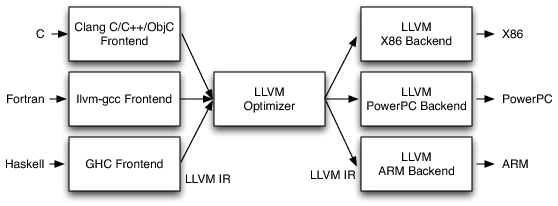
\includegraphics[width=0.8\textwidth]{LLVMCompiler1.png}
  \caption{LLVM процес компилације}
  \label{fig:grafikon}
\end{figure}

\subsection{Frond-end}
 Frond-end је задужен за парсирање, валидацију и проналазак грешака у изворном
 к\^{o}ду, затим за превођење парсираног к\^{o}да у LLVM међурепрезентацију.
 Превођење се обично извршава, прво изградњом AST-а[5], а затим 
 и превођењем AST-а у међурепрезентацију.
 У суштини сваки програмски језик, уколико имплементира front-end који може да
 изгенерише LLVM међурепрезентацију, може користити алат за оптимизацију или 
 back-end део LLVM-а.
 Постоји више пројеката који имплементирају LLVM front-end, али најбитнији су:
 
 \begin{enumerate}
 \item Clang - front-end за  C, C++ и Objective C програмске језике
 \item DragonEgg -  који користи LLVM архитектуру за оптимизацију  
 				 и генерисање машинског кода.
 \end{enumerate}

 \subsection{Алат за оптимизацију}
 Алат за оптимизацију (eng. optimizer[6]) дизајниран је тако да на улазу прима LLVM
 међурепрезентацију и изврши оптимизације над међурепрезентацијом..
 Овај алат је организован у више низова оптимизациних пролаза, тако да је излаз
 једне оптимизације улаз у другу.
 Неки од примера оптимизационих пролаза су инлајновање, елиминација мртвог кода,
 реалокација израза, размотавање петљи итд. 
 Од нивоа оптимизације зависе и оптимизациони пролази који ће бити покренути.
 У наставку ћемо приказати основне нивое оптимизације у случају Clang-a\footnote{Наведени пролази алата за оптимизацију су везани за верзију 6.0 Clang-a}
 \begin{enumerate}
 \item O0 -  основне оптимизације, корисно због брзине компајлирања и лакшег
 			дебаговања.
 			Неки од пролаза које алат за оптимизацију користи на овом нивоу су:
 			-assumption-cache-tracker -profile-summary-info -forceattrs -basiccg 		                                   always-inline -barrier.
 \item O1 - додаје велики број пролаза у односу на ниво 0, неки од пролаза су:
           lazy-value-info -jump-threading -correlated-propagation -libcalls-shrinkwrap -branch-prob -block-freq -pgo-memop-opt -tailcallelim -reassociate -loop-simplify -lcssa-verification -lcssa -scalar-evolution -loop-rotate. 
           
 \item O2 - овај ниво садржи све пролазе као ниво О1 уз додате -inline -mldst-motion -gvn -elim-avail-extern -slp-vectorizer -constmerge. У овом нивоу се избацује пролаз
 	-always-inline који ниво О0 додаје.
 \item O3 - најећи ниво оптимизације, генерише извршни фајл који се најбрже извршава
 	али по цену времена компилације. Садржи пролазе као ниво О2 уз -callsite-splitting -argpromotion.
 \end{enumerate}

\subsection{Back-end} 
LLVM back-end је фаза у којој се од међурепрезентације, која је улаз за ову фазу,
генерише машински к\^{o}д за специфичну архитектуру.
Главна компонента back-end-а је генератор к\^{o}да (eng. LLVM code generator[7]) који
користи сличан приступ као алат за оптимизацију, то јест дели генерисање машинског
к\^{o}дa на мање пролазе, који имају за циљ генерисање најбољег могућег к\^{o}да.
Неки најбитнији пролази су бирање инструкција, алокација регистара, распоређивање
(eng. scheduling).
LLVM може генерисати код за велики број архитектура, неки од њих су: x86, ARM,
PowerPC, SPARC.

\section{Предности LLVM-a}

LLVM пројекат је бесплатан и његов изворни к\^{o}д је у потпуности доступан, 
што је навело не само истраживаче са универзитета, већ и велики број компанија 
да учествују у његовом развоју, тако да данас значајан број људи активно 
учествује у одржавању и унапређивању овог пројекта.
Модуларни дизајн омогућава лако мењање постојећих алата или додавање нових.
Захваљујући овом дизајну врло лако је додати нови front-end, back-end или
оптимизациони пролаз.
Такође, LLVM подржава и:
\begin{enumerate}
\item JIT компилацију[8]
\item оптимизацију током линковања(LTO[10])
\end{enumerate}

\chapter{Оптимизација целовитог програма}

Обично изворни к\^{o}д програма делимо у више компилационих јединица (eng. compilation unit) \footnote{често се назива и јединица транслације}.
Компајлер чита фајл по фајл и за сваки генерише њему одговарајући објектни фајл,
то јест свакој компилационој јединици одговара један објектни фајл.
Овако чинимо наш к\^{o}д читљивијим, омогућавамо паралелелно компајлирање више 
фајлова али и избегавамо потребу за компајлирањем целог програма за сваку промену
у узворном к\^{o}ду.
Овакав приступ има и лошу страну, пошто компајлер преводи фајл по фајл, он нема 
информације о к\^{o}ду који се налази у другим компилационим јединицама.
Због тога што компајлер не види тела функција имплементираних у другим компилационим
јединицама, не може у потпуности да сагледа логику и изврши жељене оптимизације.
Овај проблем се може решити уз помоћ линкера,
оптимизацијом током линковања (LTO) или спајањем свих фајлова у један и извршавањем
оптимизација на једном великом фајлу (eng. unity build[9]).
\\
Сада ћемо на једном малом примеру показати због чека оптимизација целовитог програма 
може бити корисна.

\begin{lstlisting}[frame=single]
//a.h                             //a.cpp
void do_nothing();                void do_nothing(){} 

//main.cpp          
#include "a.hpp"

int main(){
    for (int i = 0; i < 1'000'000'000; i++){
        do_nothing();
    }
}
Primer 3.1
\end{lstlisting}

Видимо у примеру да функција  do{\_}nothing, као и што јој име каже, не ради ништа.
Уколико овај к\^{o}д преведемо са -О3 оптимизацијом, без оптимизације целовитог програма, добићемо следећи резултат:

\begin{lstlisting}[frame=single]
clang++  main.cpp a.cpp  -O3
time ./a.out 
real    0m1,022s
user    0m1,014s
sys     0m0,000s
\end{lstlisting}
Видимо да је рачунару било потребно више од једне секунде да изврши програм који не ради ништа.
Сада ћемо исте фајлове превести са оптимизацијом целовитог програма:
\begin{lstlisting}[frame=single]
clang++  main.cpp a.cpp  -O3 -flto=full
time ./a.out 
real    0m0,003s
user    0m0,003s
sys     0m0,000s
\end{lstlisting}

Разлика је у времену извршавања је очигледна.
Испод имамо приказ LLVM међурепрезентације без и са укљученом оптмизацијом целовитог програма
и анализираћемо разлике између њих.
\begin{lstlisting}[frame=single]
; Function Attrs: norecurse uwtable
define i32 @main() local_unnamed_addr #0 !dbg !9 {
  call void @llvm.dbg.value(metadata i32 0, 
  metadata !14, metadata !DIExpression()), !dbg !16
  br label %2, !dbg !17

; <label>:1:                                  ; preds = %2
  ret i32 0, !dbg !18

; <label>:2:                                  ; preds = %2, %0
  %3 = phi i32 [ 0, %0 ], [ %4, %2 ]
  call void @llvm.dbg.value(metadata i32 %3, 
  metadata !14, metadata !DIExpression()), !dbg !16
  tail call void @_Z10do_nothingv(), !dbg !19
  %4 = add nuw nsw i32 %3, 1, !dbg !22
  call void @llvm.dbg.value(metadata i32 %4,
  metadata !14, metadata !DIExpression()), !dbg !16
  %5 = icmp eq i32 %4, 1000000000, !dbg !23
  br i1 %5, label %1, label %2, !dbg !17, !llvm.loop
}

; Function Attrs: nounwind readnone speculatable
declare void @llvm.dbg.value(metadata, metadata, metadata)

; Function Attrs: norecurse nounwind readnone uwtable
define void @_Z10do_nothingv() local_unnamed_addr #2 
 !dbg !26 {
  ret void, !dbg !29
}
Primer 3.1 bez optimizacije celovitog programa
\end{lstlisting}


\begin{lstlisting}[frame=single]
; Function Attrs: norecurse nounwind readnone uwtable
define dso_local i32 @main() local_unnamed_addr #0 
!dbg !9 {
  call void @llvm.dbg.value(metadata i32 0, 
  metadata !14, metadata !DIExpression()), !dbg !16
  ret i32 0, !dbg !17
}

; Function Attrs: nounwind readnone speculatable
declare void @llvm.dbg.value(metadata, metadata, metadata)

Primer 3.1 sa optimizacijom celovitog programa
\end{lstlisting}

У примеру где није укључена оптимизација целовитог програма компајлер не зна како
изгледа функција do{\_}nothing и он мора милион пута у пељи да је позива.
Када је укључена оптимизација целовитог програма компајлер види тело те функције,
и види да она не ради ништа, тако да може да оптимизује не само позивање те функције,
односно да је инлајнује, већ може да уклнони комплетну петљу, јер после инлајновања
функције do{\_}nothing тело петље остаје празно.
Видимо да је елиминисана и функција do{\_}nothing из извршног програма и да је унутар
main функције остала само повратна вредност, што овај програм само и ради.
О инлајновању и елиминацији мртвог к\^{o}д биће више речи у наставку.

\section{Ортимизација током линковања}


Захваљујући модуларном дизајну LLVM-a и чињеници да можемо компајлирати део к\^{o}да,
сачувати резултат и наставити компилацију касније без губитака информација
слику 2.1 можемо допунити додавањем линкера и оптимизацијама током процеса линковања.

\begin{figure}[!ht]
  \centering
  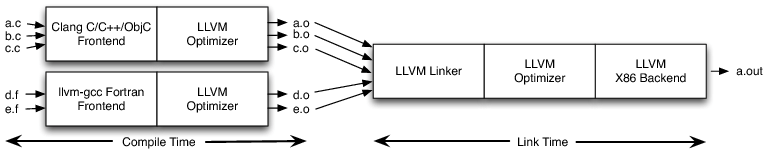
\includegraphics[width=0.8\textwidth]{LTO.png}
  \caption{LLVM процес компилације са подршком линкера}
  \label{fig:grafikon}
\end{figure}


У наставку ћемо објаснити због чега је линкер користан у оптимизацији целовитог програма.

Главни задатак линкера је да све објектне фајлове споји у један фајл, извршни фајл
или дељену библиотеку. 
Да би испунио овај задатак линкер прво мора да извши реалокацију симбола и резолуцију
симбола.
Симболи могу бити глобалне променљиве, функције, класе итд. 
Сваки објектни фајл садржи табелу симбола у којој се налазе сви симболи који 
могу бити дефинисани у истом објектном фајлу или у неком другом.
Уколико симбол није дефинисан унутар објектног фајла он ће у табели симбола бити
означен као "extern", у супротном биће означен као "import".
Да би се успешно превео програм у извршни фајл, линкер мора да пронађе све 
недостајуће симболе у свим објектним фајловима и да упише њихове адресе (такође задатак
линкера је да и неким импортованим симбола промени адресу, уколико је компајлер то назначио),
то јест да изврши резолуцију и реалокацију симбола.
Због ових својстава линкер има круцијалну улогу у оптимизацији целовитог програма, јер
има увид у све табеле симбола и алат за оптимизацију може то искористити за оптимизације
делова к\^{o}да који су му пре били "невидљиви". 
\\
У наставку приказаћемо интеракцију између линкера и алата за оптимизацију.
Оптимизација током линковања у LLVM инфраструктури садржи четири фазе:
\begin{enumerate}
\item Читање битк\^{o}д фајлова
\item Резолуција симбола
\item Оптимизовање биткод фајлова
\item Резолуција симбола након оптимизације
\end{enumerate}

\subsection{Читање битк\^{o}д фајлова}
Сви објектни фајлови долазе до линкера, који из њих чита и сакупља информације
о симболима, који су присутни у фајловима.
Ови фајлови могу бити у форми LLVM битк\^{o}д фајлова или стандардних објектних
фајлова (eng. native object files).
Линкер већ има могућност за третирање објектних фајлова, да би могао
правилно да чита и LLVM битк\^{o}д фајлове потребна му је помоћ, а то му омугућава
алат под називом libLTO[11].
libLTO је библиотека који је намењена за коришћење од стране линкера.
libLTO има стабилан интерфејс, тако да је могуће користити
LLVM алат за оптимизацију, без потребе за излагањем интерног LLVM к\^{o}да.
Такође, још једна предност овог алата је то што можемо мењати LLVM LTO к\^{o}д независно
од линкера, то јест не морамо за сваку промену к\^{o}да који имплементира
оптимизације мењати и линкер.
\\
Да се вратимо на фазу читања битк\^{o}д фајлова, уколико линкер добије
објектни фајл, он већ зна да чита тај фајл и додаће симболе у глобалну табелу симбола.
Уколико је у питању LLVM битк\^{o}д фајл, линкер ће позвати функције \\
lto{\_}module{\_}get{\_}symbol{\_}name и 
lto{\_}module{\_}get{\_}symbol{\_}attribute 
libLTO алата да би добио све дефинисане  симболе, затим ће те симболе, 
као у случају стандардног објектног фајла, додати у глобалну табелу симбола.

\subsection{Резолуција симбола}
Као што је већ објашњено изнад, линкер покушава да разреши све симболе помоћу
глобалне табеле симбола.
Уколико је укључена опција елиминације мртвог кода, која је подразумевано укључена
уколико се користи оптимизација током линковања, линкер чува листу симбола који
су коришћени у осталим објектним фајловима, такозвани живи симболи.

\subsection{Оптимизација битк\^{o}д фајлова} 
У овој фази линкер користи информације из глобалне табеле симбола, и пријављује
живе симболе алату за оптимизацију
lto{\_}codegen{\_}add{\_}must{\_}preserve{\_}symbol функцијом.
Затим линкер позива алат за отимизацију и генератор к\^{o}да над битк\^{o}д фајловима
функцијом lto{\_}codegen{\_}compile чији је резулат објектни фајл
који настао спајањем више битк\^{o}д фајлова, са примењеним оптимизацијама на њима.
Примећујемо да је оптимизације могуће извршити искључиво на битк\^{o}д фајловима,
то јест објектни фајлови се не оптимизују.

\subsection{Резолуција симбола након оптимизације}
У овој фази линкер чита оптимизоване објектне фајлове и ажурира табелу симбола уколико 
има неких промена. На пример уколико је укључена елиминација мртвог к\^{o}да,
линкер може да избаци неке симболе из табеле.
У овој фази сви фајлови су објектни фајлови и линковање се наставља
по старом принципу, као да никада нису ни постојали битк\^{o}д фајлови.

\section{Оптимизација целовитог програма без подршке линкера}
\begin{figure}[!ht]
  \centering
  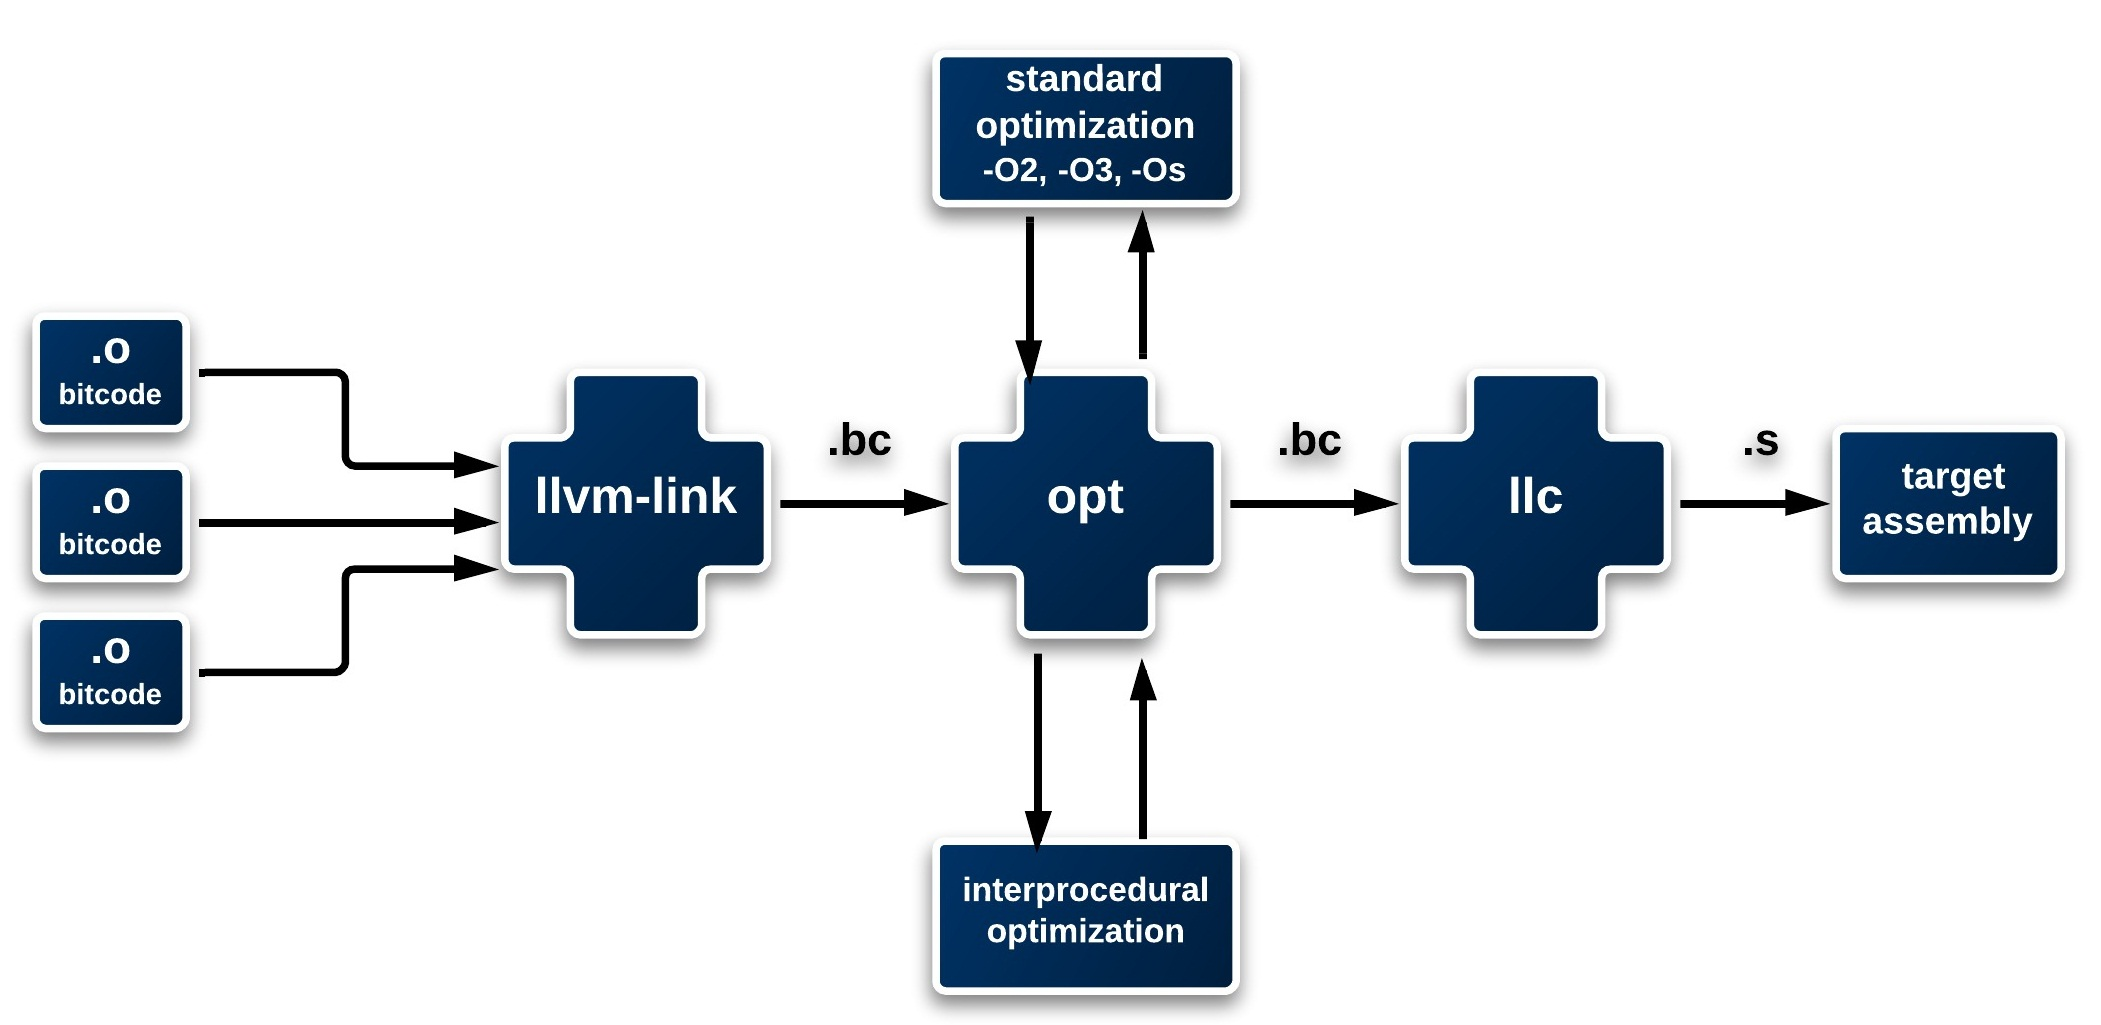
\includegraphics[width=0.8\textwidth]{llvm_link.png}
  \caption{LLVM процес компилације без подршке линкера}
  \label{fig:grafikon}
\end{figure}

Приступ отимизације целовитог програма са линкером захтева Gold[12] линкер,
који у себи има подршку за libLTO библиотеку.
На неким системима овај линкер није доступан и ту је немогуће извршити стандардну
оптимизацију током линковања.
Алтернативни приступ је спајање свих LLVM битк\^{o}д фајлова у један битк\^{o}д фајл
и извршавање оптимизација над тим фајлом.
Ово је могуће захваљујући LLVM алату llvm-link[13].
\\
Овим приступом добијамо исте перфомансе као са приступом где имамо подршку линкера,
са тим што овај приступ неће радити уколико сви фајлови нису  битк\^{o}д фајлови,
односно не ради са објектним фајловима.


\section{Инлајновање функција}

Уобичајена пракса у програмирању је издвајање к\^{o}да који се понавља у 
засебне функције.
Издвајање к\^{o}да је корисно зато што на тај начин избацујемо копирање
истог к\^{o}да на више места у програму.
На тај начин не само да повећавамо читљивост програма, већ и смањујемо
могућност грешака, које су честе при копирању  к\^{o}да.
Са друге стране, позиви функција могу бити захтевни што се тиче времена извршања.
Када се функција позове долази до креирања новог стек оквира, померања показивача
инструкција на почетак те функције, чувања тренутног стања позиваоца функције у 
регистрима и слично.
Такође,  к\^{o}д функције може бити ван кеша инструкција, што може битно
утицати на време извршавања програма.
Решење ових проблема је инлајновање функција (eng. function inlining[14]).
Инлајновање је замена позива функције у компајлираном к\^{o}ду
целокупним телом позване функције.
Поред тога што инлајновање елинише утрошено време позива функције, оно такође
омогућава компајлеру да генерише оптималнији к\^{o}д.
Пошто је цео к\^{o}д функције уметнут, компајлер може извршити оптимизације у већем
блоку, што некада може довести до значајних убрзања.
Видели смо да инлајновање функција може бити корисно и намеће се логично питање-
када можемо извршити инлајновање?
Неке функције можемо одмах елиминисати из списка кандидата за инлајновање, уколико имамо дељену динамичку библиотеку, ми немамо
информацију о к\^{o}ду функције тако да је не можемо инлајновати.
Сличан проблем је са функцијама које се налазе у другим објектним фајловима, али за
овај проблем постоји решење, а то је оптимизација целовитог програма.
Уколико је оптимизација целовитог програма укључена, компајлер може видети
к\^{o}д функција из других објектних фајлова и евенутално их инлајновати.
Такође, немогуће је инлајновати функције које садрже инструкције индиректног
гранања(eng. indirect branch instructions[15]) јер у том случају, уколико би 
инлајновали функцију, индиректне гране би нас довеле до неочекиваних инструкција
у програму.
\par 
Видели смо да инлајновање има велики број предности, али да га није могуће увек
урадити, да ли онда увек инлајновати када је то могуће?
Наравно, одговор је не. 
Поред великог броја предности, инлајновање има и неке мане.
Једна од мана је повећање величине извршног фајла, поготово када функције имају
велики број инструкција.
Видимо да ипак мора да постоји компромис између перфоманси програма и величине
извршног фајла.
Такође, функције са великим бројем инструкција могу да утичу на перфомансе, тако
што утичу на кеш инструкција, јер велики број инструкција руши локалност референци. 
На пример уколико инлајнујемо функцију са великим бројем инструкција 
унутар петље, врло је могуће да тај блок више не стаје у кеш инструкција,
и онда при свакој итерацији петље имамо промашај кеша. Због тога се
обично избегава инлајновање оваквих функција.
Због свега наведеног за инлајновање користимо хеуристике, преко којих одређујемо
да ли неку функцију треба инлајновати или не.
Битне информације које користе хеуристике су колико функција има инструкција,
колико пута се позива у току програма, да ли је функција коришћена у осталим
објектним фајловима и слично.
Поред ове статичке анализе функција, где користимо фиксиране границе(eng. threshold)
за број иснтрукција, позива итд. и тако одређујемо да ли треба да инлајнујемо функцију,
постоји и динамчка анализа.
Динамичка анализа користи информације које се добијају приликом профајлирања програма.
На овај начин можемо добити прецизније информације и самим тим боље перфомансе програма после оптимизације,
али само у случају да тестно окружење програма симулира реалну ситуацију у којој
ће се програм извршавати.
У супротном можемо добити лошије перфомансе него статичком анализом.
Профајлирањем можемо открити делове к\^{o}да који се чешће извршавају, и компајлер 
поклања посебну пажњу оптимизовању и инлајновању тих делова, јер уколико се неке
функције скоро никада не позивају, инлајновањем нећемо добити никакве предности
у перфомансама, само можемо повећати величину извршног фајла.	
Програмер може у извнорном  к\^{o}ду сигнализирати компајлеру да изврши инлајновање
атрибутом always{\_}inline, на системима Unix, али ни то не гарантује да ће на крају
функција заиста бити инлајнована.
\par
Приказаћемо један пример где је могуће извршити инлајновање уколико
је укључена оптимизација целовитог програма.

\begin{lstlisting}[frame=single]
//square.hpp           
int square(int);         
    					
//square.cpp				
int square(int a){
    return a *a;
}

//main.cpp
#include "square.hpp"
#include <iostream>

int main(){
    int result = 0;
    
    for (int i = 0; i < 100; i++){
        result+= square(i);
    }
    std::cout << result;
}

Primer 3.3.1
\end{lstlisting}

Сада ћемо видети разлике LLVM међурепрезентације без и са оптимизацијом
целовитог програма у примеру 3.3.1.

\begin{lstlisting}[frame=single]
 Function Attrs: norecurse uwtable
define i32 @main() local_unnamed_addr #4 !dbg !966 {
  call void @llvm.dbg.value(metadata i32 0, 
  metadata !968, metadata !DIExpression()), !dbg !971
  call void @llvm.dbg.value(metadata i32 0, 
  metadata !969, metadata !DIExpression()), !dbg !972
  br label %3, !dbg !973

; <label>:1:                              ; preds = %3
  %2 = tail call dereferenceable(272) 
  %"class.std::basic_ostream"* 
  @_ZNSolsEi(%"class.std::basic_ostream"* 
  nonnull @_ZSt4cout, i32 %7), !dbg !974
  ret i32 0, !dbg !975

; <label>:3:                              ; preds = %3, %0
  %4 = phi i32 [ 0, %0 ], [ %8, %3 ]
  %5 = phi i32 [ 0, %0 ], [ %7, %3 ]
  call void @llvm.dbg.value(metadata i32 %5, 
  metadata !968, metadata !DIExpression()), !dbg !971
  call void @llvm.dbg.value(metadata i32 %4, 
  metadata !969, metadata !DIExpression()), !dbg !972
  %6 = tail call i32 @_Z6squarei(i32 %4), !dbg !976
  %7 = add nsw i32 %6, %5, !dbg !979
  %8 = add nuw nsw i32 %4, 1, !dbg !980
  call void @llvm.dbg.value(metadata i32 %8, 
  metadata !969, metadata !DIExpression()), !dbg !972
  call void @llvm.dbg.value(metadata i32 %7, 
  metadata !968, metadata !DIExpression()), !dbg !971
  %9 = icmp eq i32 %8, 100, !dbg !981
  br i1 %9, label %1, label %3, !dbg !973, !llvm.loop !982
}

; Function Attrs: nounwind readnone speculatable
declare void @llvm.dbg.value(metadata, 
metadata, metadata) #5

declare dereferenceable(272)
 %"class.std::basic_ostream"* 
 @_ZNSolsEi(%"class.std::basic_ostream"*, i32) 
 local_unnamed_addr #1

; Function Attrs: nounwind readnone uwtable
define i32 @_Z6squarei(i32) local_unnamed_addr
 #6 !dbg !984 {
  call void @llvm.dbg.value(metadata i32 %0, 
  metadata !986, metadata !DIExpression()), !dbg !987
  %2 = mul nsw i32 %0, %0, !dbg !988
  ret i32 %2, !dbg !989
}
Primer 3.3.1 bez optimizacije celovitog programa
\end{lstlisting}

\begin{lstlisting}[frame=single]
; Function Attrs: norecurse uwtable
define dso_local i32 @main() local_unnamed_addr 
#4 !dbg !966 {
  call void @llvm.dbg.value(metadata i32 0, 
  metadata !968, metadata !DIExpression()), !dbg !971
  call void @llvm.dbg.value(metadata i32 0, 
  metadata !969, metadata !DIExpression()), !dbg !972
  %1 = tail call dereferenceable(272) 
  %"class.std::basic_ostream"* 
  @_ZNSolsEi(%"class.std::basic_ostream"* nonnull 
  @_ZSt4cout, i32 328350), !dbg !973
  ret i32 0, !dbg !974
}

; Function Attrs: nounwind readnone speculatable
declare void @llvm.dbg.value(metadata,
 metadata, metadata) #5

declare dereferenceable(272) 
%"class.std::basic_ostream"* 
@_ZNSolsEi(%"class.std::basic_ostream"*, i32) 
local_unnamed_addr #1

Primer 3.3.1 sa optimizacijom celovitog programa
\end{lstlisting}

Ако погледамо међурепрезентацију без оптимизације целовитог програма видимо да је она јако
слична изворном к\^{o}ду, компајлер не види тело функције square, тако да не може неке 
значајније оптимизације да изврши.
Са друге стране, када је укључена оптимизација целовитог програма, компајлер
успева да инлајнује функцију.
Овим се компајлер не само решава трошкова позива функција, већ омогућава и остале оптимизације.
Зато што сада имамо тело функције у блоку петље, компајлер увиђа да се петља извршава константан
број пута и да нема потребе стално израчунавати исту приликом покретања програма, већ вредност
променљиве result може да се израчуна у току компилације програма, самим тим се решавамо петље и к\^{o}да око ње.
У позиву std::cout функције видимо резултат израчунавања :
\begin{lstlisting}[frame=single]
tail call dereferenceable(272) %"class.std::basic_ostream"*
@_ZNSolsEi(%"class.std::basic_ostream"
* nonnull @_ZSt4cout, i32 328350)
\end{lstlisting}
Такође, више нема потребе за постојањем функције square(више се нигде не користи)
и она је избрисана из извршног фајла.



\section{Елиминација мртвог к\^{o}да}

Елиминација мртвог к\^{o}да(eng. dead code elimination[16]) је компајлерска 
оптимизација која елиминише к\^{o}д који не утиче на резултат извршавања
програма.
Уклањање мртвог к\^{o}да има многе предности: смањује величину извршног програма,
побољшава локалност инструкција, уклањањем непотребних инструкција такође
повећава брзину извршавања програма.
Без укључене оптимизације целовитог програма компајлер може да елинише локалне
променљиве, инлајноване статичке функције као и статичке глобалне променљиве.
То ради једноставним праћењем позива свих статичких глобала и сврставањем истих
у живе или мртве скупове, у зависности да ли се глобал користи или не.
Све глобале из мртвог скупа, на крају оптимизационих пролаза, можемо елиминисати.
Са укљученом оптимизацијом целовитог програма можемо избацити не само статичке
глобалне променљиве или функције, него све глобале који се не користе.
Овај поступак се извршава током линковања и описан је у секцији  3.1.

Пример елиминације мртвог мртвог к\^{o}да смо већ видели у претходном примеру
у којем је компајлер уклонио функцију square јер се није користила. Наредни
програм ће ово приказати на неколико очигледнијих примера:

\begin{lstlisting}[frame=single]
//a.hpp
int foo1(void);
void foo2(void);
void foo4(void);

//a.cpp
#include "a.hpp"

static signed int i = 0;

void foo2(void) {
  i = -1;
}

static int foo3() {
  foo4();
  return 10;
}

int foo1(void) {
  int data = 0;

  if (i < 0)
    data = foo3();

  data = data + 42;
  return data;
}

//main.cpp
#include <iostream>
#include "a.hpp"

void foo4(void) {
  std::cout << ("Hi\n");
}

int main() {
  return foo1();
}

Primer 3.4.1
\end{lstlisting}

\begin{lstlisting}[frame=single]
 Function Attrs: uwtable

declare dereferenceable(272) 
%"class.std::basic_ostream"* @_ZSt16__
ostream_insertIcSt11char_traitsIcEERSt13basic_
ostreamIT_T0_ES6_PKS3_l
(%"class.std::basic_ostream"* 
dereferenceable(272), i8*, i64) local_unnamed_addr #1

; Function Attrs: uwtable
define void @_Z4foo4v() local_unnamed_addr #0 !dbg !983 {
  call void @llvm.dbg.value(metadata 
  %"class.std::basic_ostream"* @_ZSt4cout, 
  metadata !984, metadata !DIExpression()), !dbg !1048
  call void @llvm.dbg.value(metadata i8* 
  getelementptr inbounds ([4 x i8], [4 x i8]*
   @.str, i64 0, i64 0), 
  metadata !993, metadata !DIExpression()), !dbg !1050
  %1 = tail call dereferenceable(272) 
  %"class.std::basic_ostream"*
   @_ZSt16__ostream_insertIcSt11char_
  traitsIcEERSt13basic_ostreamIT_T0_ES6_PKS3_l
  (%"class.std::basic_ostream"* nonnull dereferenceable(272) 
  @_ZSt4cout, i8* nonnull getelementptr 
  inbounds ([4 x i8], [4 x i8]* @.str, i64 0, i64 0), 
  i64 3), !dbg !1051
  ret void, !dbg !1053
}

; Function Attrs: norecurse uwtable
define i32 @main() local_unnamed_addr #5 !dbg !1054 {
  %1 = tail call i32 @_Z4foo1v(), !dbg !1055
  ret i32 %1, !dbg !1056
}

; Function Attrs: norecurse nounwind uwtable
define void @_Z4foo2v() local_unnamed_addr #6 !dbg !1057 {
  store i1 true, i1* @_ZL1i, align 4
  ret void, !dbg !1058
}

; Function Attrs: uwtable
define i32 @_Z4foo1v() local_unnamed_addr #0 !dbg !1059 {
  call void @llvm.dbg.value(metadata i32 0,
   metadata !1061, metadata !DIExpression()), !dbg !1062
  %1 = load i1, i1* @_ZL1i, align 4
  br i1 %1, label %2, label %3, !dbg !1063

; <label>:2:                              ; preds = %0
  tail call void @_Z4foo4v(), !dbg !1064
  call void @llvm.dbg.value(metadata i32 10, 
  metadata !1061, metadata !DIExpression()), !dbg !1062
  br label %3, !dbg !1068

; <label>:3:                              ; preds = %2, %0
  %4 = phi i32 [ 52, %2 ], [ 42, %0 ]
  call void @llvm.dbg.value(metadata i32 %4, 
  metadata !1061, metadata !DIExpression()), !dbg !1062
  ret i32 %4, !dbg !1069
}

Primer 3.4.1 bez optimizacije celovitog programa
\end{lstlisting}


\begin{lstlisting}[frame=single]
; Function Attrs: norecurse nounwind readnone uwtable
define dso_local i32 @main() local_unnamed_addr #4 
!dbg !982 {
  ret i32 42, !dbg !983
}
Primer 3.4.1 sa optimizacijom celovitog programa
\end{lstlisting}

У примеру без оптимизације целовитог програма, видимо да је компајлер инлајновао
функцију foo3 и она се не налази унутар извршног фајла.
Компајлер је успео да елиминише функцију јер је она статичка, али остале нису
тако да се оне налазе у извршном фајлу.
Видимо да је и к\^{o}д међурепрезентације сличан изворном, тако да компајлер поред
инлајновања, није успео да изврши неке веће оптимизације.
\\
Са друге стране, у примеру са оптимизацијом целовитог програма, видимо да је у
извршном фајлу остала само main функција, која враћа вредност 42.
Да бисмо утврдили како се то догодило, проћи ћемо кроз цео процес оптимизације овог 
програма, са укљученом оптимизацијом целовитог програма.
Линкер прво препознаје да се функција foo2 не користи нигде у програму, шаље ту
информацију компајлеру(конкретно алату за оптимизацију) и он је брише.
Чим обрише функцију, алат за оптимизацију види да услов i < 0 никада није испуњен,
тако да може да обрише и тај део к\^{o}да али и функцију foo3, јер се она сада
више неће користити.
Линкер сада препознаје да се функција foo4 не користи више тако да се и она брише.
На крају остаје само функција foo1 која увек враћа вредност 42, то алат за оптимизацију
препознаје, инлајнује је, брише и враћа вредност 42 као повратну вредност функције
main.

\section{Девиртуализација}
 Девиртуализација(eng. devirtualization[17]) је поступак замене виртуелних позива
 функција директним позивима.
 Виртуелни позиви функција су неколико пута спорији од директних, што у системима
 у којима је брзина извршавања програма кључна може да буде велики проблем.
 Због тога је пожељно извршити девиртуелизацију када је то могуће.
 Девиртуализација се најефикасније може извршити уз помоћ оптимизације целовитог
 програма, али постоје и случајеви у којима је могуће извршити девиртуализацију 
 и без оптимизације целовитог програма.
 За почетак ћемо се позабавити тим случајевима.
 
 \subsection{Познат динамички тип објекта}
 Уколико нам је познат динамички тип објекта при компајлирању, компајлер може 
 да девиртуализује позив функције.
 
 \begin{lstlisting}[frame=single]
#include <iostream>
struct Base{
    virtual int f(){return 1;}
};

struct Derived : Base{
    int f() override {return 2;}
};

int main(){
    Derived d;
    Base * b = new Base();
    std::cout << b->f();
    std::cout << d.f();  
}
 Primer 3.5.1
 \end{lstlisting}
 
 \begin{lstlisting}[frame=single]
; Function Attrs: norecurse uwtable
define i32 @main() local_unnamed_addr #4 !dbg !964 {
  call void @llvm.dbg.value(metadata %struct.Derived* undef,
   metadata !966, metadata !DIExpression()), !dbg !985
  %1 = tail call dereferenceable(272) 
  %"class.std::basic_ostream"* @_ZNSolsEi
  (%"class.std::basic_ostream"* nonnull @_ZSt4cout, i32 1), 
  !dbg !986
  call void @llvm.dbg.value(metadata %struct.Derived* undef, 
  metadata !966, metadata !DIExpression()), !dbg !985
  %2 = tail call dereferenceable(272) 
  %"class.std::basic_ostream"* @_ZNSolsEi
  (%"class.std::basic_ostream"* nonnull @_ZSt4cout, 
  i32 2), !dbg !987
  ret i32 0, !dbg !988
}
Primer 3.5.1 LLVM
 \end{lstlisting}
 
 Као што видимо у примеру изнад, компајлер успешно девиртуализује и инлајнује ове функције јер види да је променљива b иницијализована на new Base(), 
 док променљива је променљива d типа Derived, па ту и не постоји виртуелни позив
  и поред тога што је чланска функција f виртуелна.
 \footnote{Када променљива није показивчког или референцног типа 
  компајлер зна да позив не може бити виртуелан.}
 
 \subsection{Кључна реч final}
 У програмском језику C++ kључна реч final означава да функција не може бити 
 препревљена у изведеној класи (уколико се кључна реч final налази у потпису функције)
 или да се из те класе не може извести нова класа (уколико се кључна реч final
 налази у потпису класе).
 Искористићемо пример сличан примеру 3.5.1:
 
\begin{lstlisting}[frame=single]
struct Base{
    virtual int f(){return 1;}
};

struct Derived final : Base{
    int f() override {return 2;}
};
int func(Derived *d){
    return d->f();
}

Primer 3.5.2
\end{lstlisting}
 
 За разлику од примера 3.5.1 овде смо структуру Derived обележили кључном 
 речју final.
 То говори комапјлеру да ни у овој, али ни у било којој другој јединици превођења, 
 не може постојати структура која је изведена из структуре Derived.
 То сазнање омогућава компајлеру да изврши девиртуализацију позива функције f().
 Примећујемо када не бисмо експлицитно обележили  Derived са final девиртуализација
 не би била могућа, јер компајлер не може да зна да ли у некој другој јединици превођења
 постоји структура изведена из структуре Derived и самим тим преправљена функција(eng. override).
 
 \subsection{Унутрашња видљивост}
 Када кажемо да нека променљива или функција има унутрашњу видљивост
 (eng. internal linkage[18]) то значи да је она видљива само унутар своје јединице
 транслације.
 Што значи да уколико имамо структуру, или класу, која има унутрашњу видљивост,
 комапјлер може девиртуализовати позив функције јер је сигуран да она неће моћи бити
 преправљена.
 Видимо да је овај принцип сличан као додавање кључне речи  final.
 Један једноставан начин да наша класа добије унутрашњу видљивост јесте смештање исте
 у безимени простор имена(eng. unnamed namespace[19]).
 Овај принцип приказан је у примеру 3.5.3.
 
 \begin{lstlisting}[frame=single]
namespace{
struct Base{
    virtual int f(){return 1;}
};

struct Derived : Base{
    int f() override {return 2;}
};
}
Primer 3.5.3
\end{lstlisting}
 
\subsection{Девиртуализација помоћу оптимизације целовитог програма}
 
 Видели смо ситуације када компајлер без оптимизације целовитог програма може да
 изврши девиртуализацију.
 У већини ситуација нећемо наилазити на тако једноставне случајеве, а и често ће
 дефиниције виртуелних функција бити у другим јединицама транслације.
 Због тога што компајлер види цео програм, када је укључена оптимизација
 целовитог програма, он види и функције и класе, тако да може да изврши
 девиртуализацију агресивније.
 Погледајмо следећи пример, који има само 1 изворни фајл.
 \begin{lstlisting}[frame=single]
#include <iostream>
struct Base
{
  virtual int f() { return 1; }
};

struct Derived : public Base
{
  int f() override { return 2; }
};

int g(Derived *obj)
{
  return obj->f();
}

int main()
{
  Derived *obj = new Derived();
  std::cout << g(obj);
}
Primer 3.5.4
\end{lstlisting}
	
\begin{lstlisting}[frame=single]
; Function Attrs: uwtable
define i32 @_Z1gP7Derived(%struct.Derived*)
 local_unnamed_addr #0 !dbg !964 {
  call void @llvm.dbg.value(metadata %struct.Derived* %0,
   metadata !985, metadata !DIExpression()), !dbg !986
  %2 = bitcast %struct.Derived* %0 to i32 
  (%struct.Derived*)***, !dbg !987
  %3 = load i32 (%struct.Derived*)**, 
  i32 (%struct.Derived*)*** %2, 
  align 8, !dbg !987, !tbaa !988
  %4 = load i32 (%struct.Derived*)*, 
  i32 (%struct.Derived*)** %3, 
  align 8, !dbg !987
  %5 = tail call i32 %4(%struct.Derived* %0), !dbg !987
  ret i32 %5, !dbg !991
}

; Function Attrs: nounwind readnone speculatable
declare void @llvm.dbg.value(metadata,
 metadata, metadata) #4

; Function Attrs: norecurse uwtable
define i32 @main() local_unnamed_addr #5 
!dbg !992 {
  %1 = tail call dereferenceable(272) 
  %"class.std::basic_ostream"* 
  @_ZNSolsEi(%"class.std::basic_ostream"* nonnull 
  @_ZSt4cout, i32 2), !dbg !995
  ret i32 0, !dbg !996
}
Primer 3.5.4 bez optimizacije celovitog programa
\end{lstlisting}

\begin{lstlisting}[frame=single]
; Function Attrs: norecurse uwtable
define dso_local i32 @main() local_unnamed_addr #4 !dbg !964 {
  %1 = tail call dereferenceable(272) 
  %"class.std::basic_ostream"* 
  @_ZNSolsEi(%"class.std::basic_ostream"* nonnull
   @_ZSt4cout, i32 2), !dbg !984
  ret i32 0, !dbg !985
}
Primer 3.5.4 sa optimizacijom celovitog programa
\end{lstlisting}

У примеру без оптимизације целовитог програма видимо инструкције за узимање вредности
виртуелног показивача и позивање виртуелне функције, што значи да компајлер није успео
да девиртуализује позив иако види тело функције и класе.
То се дешава због тога што компајлер не зна да ли у некој другој јединици транслације
постоји класа која је изведена из класе Derived и због тога не може да изврши
оптимизације.
Са укљученом оптимизацијом целовитог програма компајлер види да не постоји класа
изведена из класе Derived и компајлер успешно девиртуализује, а затим и инлајнује
позив функције. 
 
 \chapter{ThinLTO}
 
 У претходном поглављу видели смо како оптимизација целовитог програма може значајно
 побољшати перфомансе нашег програма.
 Такође, видели смо како је имплементирана стандардна оптимизација током линковања,
 укратко линкер добија битк\^{o}д фајлове, уместо објектних фајлова, затим се ти
 битк\^{o}д фајлови спајају у један и над тим фајлом се врше све оптимизације.
 
\begin{figure}[!ht]
  \centering
  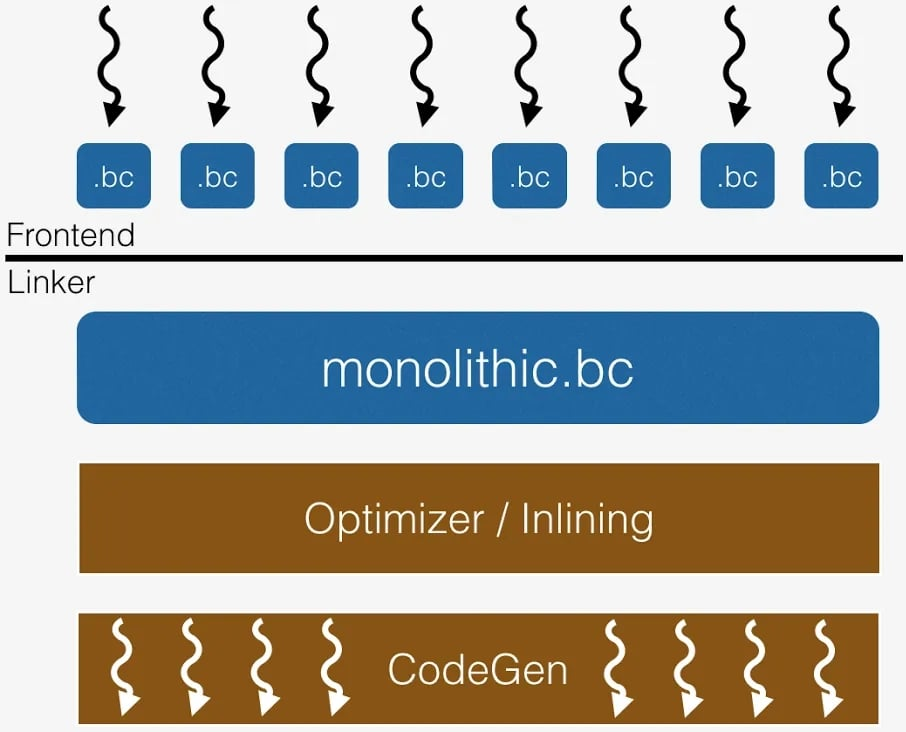
\includegraphics[width=0.8\textwidth]{LTO_normal.png}
  \caption{Стандардни процес оптимизације током линковања}
  \label{fig:grafikon}
\end{figure}

Стандардни приступ има неколико мана.
Први проблем је то што губимо предности паралелног компајлирања, која постоји 
када није активна оптимизација целовитог програма.
Као што видимо на слици 4.1 постоји паралелно превођење изворних фајлова у 
битк\^{o}д фајлове али због спајања свих фајлова у један велики битк\^{o}д фајл,
ту предност касније губимо зато што све оптимизације над тим фајлом морају 
да се раде без могућности парелелизације.
Због тога компајлирање траје много дуже него без оптимизације целовитог програма.
Такође, за сваку промену у било ком изворном фајлу, ми поново морамо испочетка
вршити све оптимизације на обједињеном фајлу, што поново изузетно утиче не време
превођења.
Још један велики проблем овог приступа је то што сада у меморији морају да се налазе  међурепрезентације свих компилационих јединица одједном, спојене
у једну, често је немогуће извршити оптимизацију целовитог програма, поготово на 
машинама које немају велику радну меморију.
Приступ за решавање ових проблема је  ThinLTO[20].
\par ThinLTO је нови приступ који омогућава сличне перфомансе при превођењу
као када није укључена оптимизација целовитог програма, док задржава већину
оптимизација и самим тим перфоманси извршног фајла као регуларна оптимизација
целовитог програма.
При ThinLTO оптимизацији уместо учитавања битк\^{o}д фајлова и спајања у један,
већ за сваку јединицу транслације и сваку функцију или глобал у њој, чува кратак
резиме за анализу у кораку линковања. 
Кључна оптимизација коју ThinLTO омогућава је убацивање само оних функција које
су потребне конкретном битк\^{o}д фајлу и које ће бити инлајноване у том  битк\^{o}д фајлу.
И тај поступак радимо за сваки  битк\^{o}д фајл, што значи да нема спајања, већ се и
даље поступак  извршава паралелно.
ThinLTO процес оптимизације целовитог програма је подељен на 3 фазе:
\begin{enumerate}
\item Превођење - генеришу се међурепрезензације као и случају стандардног процеса
	оптимизације целовитог програма, са тим што сада имамо и резиме уз сваку
	међурепрезентацију
\item Линковање - линкер комбинује резимее из прошлог корака и врши анализу
\item Бекенд - паралелна оптимизација и генерисање к\^{o}да
\end{enumerate}
 
\begin{figure}[!ht]
  \centering
  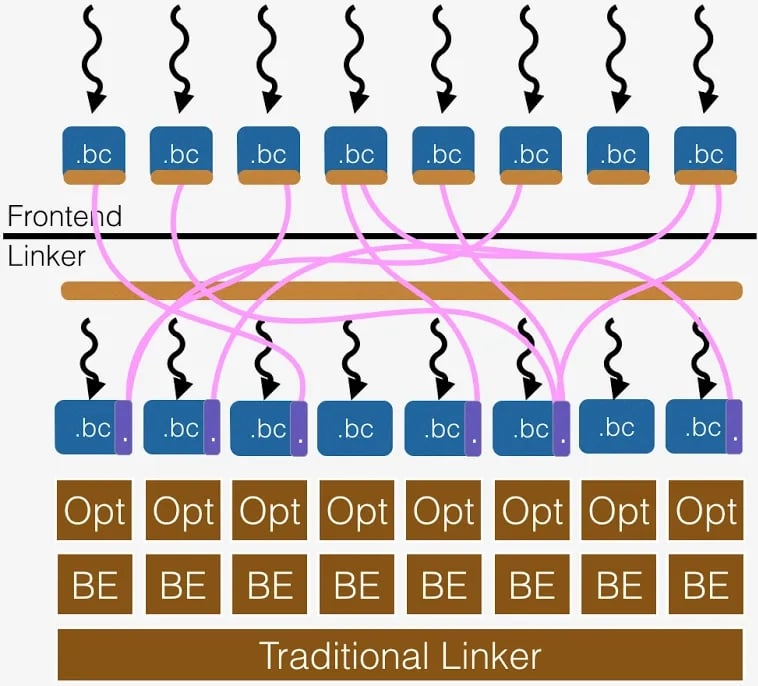
\includegraphics[width=0.8\textwidth]{LTO_thin.png}
  \caption{ThinLTO процес оптимизације}
  \label{fig:grafikon}
\end{figure}

Кључни део ThinLTO оптимизације се дешава у првој фази, а то су креирања резимеа.
Свака глобална променљива и функција се налазе у резимеу, за ту јединицу транслације.
Резиме садржи по једно поље за сваки симбол и у том пољу
се налазе подаци који описују тај симбол.
На пример, за функцију, у пољу унутар резимеа може да стоји њена видљивост, 
број инструкција које функција садржи, информације за профајлирање уколико су потребне
и слично.
Додатно, свака референца према другом симболу(позив друге функције, узимање адресе,
приступање глобалу) се записује у резиме и тако се гради граф контроле тока(eng. call graph).
Ове информације омогућавају креирање комплетног графа током фазе линковања.
ThinLTO је једноставно активирати, само је потребно додати  -flto=thin у командној линији
приликом компајлирања.
\\
Сада ћемо приказати разлику између перфоманси, меморијских захтева као и времена
компајлирања између оптимизације током линковања и ThinLTO-а.
Слике су преузете са чланка ThinLTO: Scalable and Incremental LTO[21].

\begin{figure}[!ht]
  \centering
  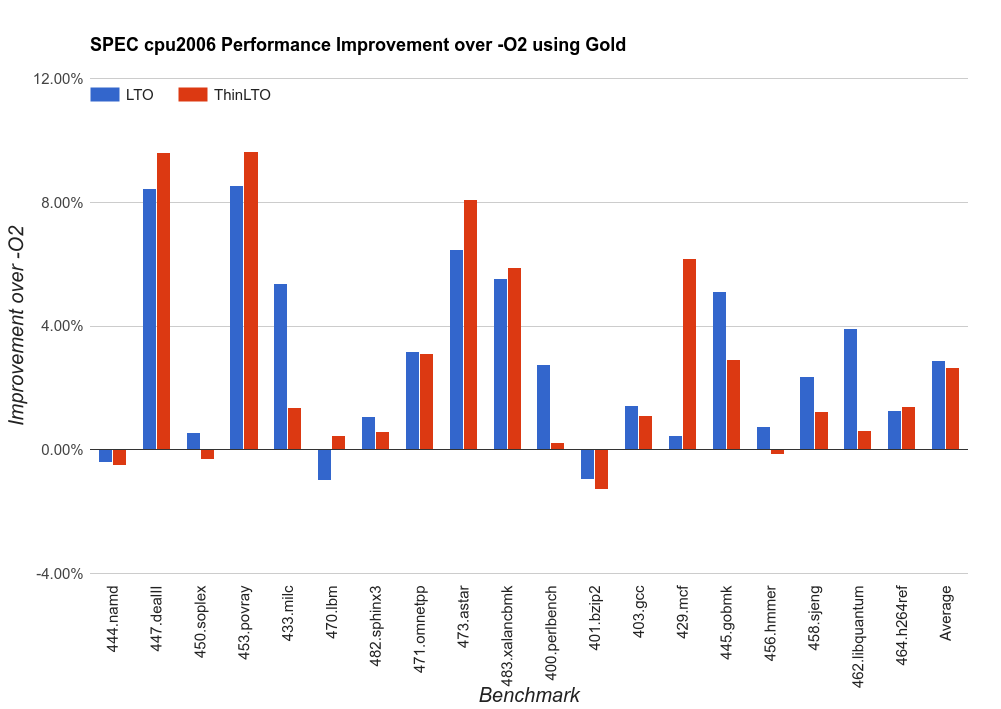
\includegraphics[width=0.8\textwidth]{thin_perfomance.png}
  \caption{Разлика у перфомансама између ThinLTO и регуларне оптимизације током линковања }
  \label{fig:grafikon}
\end{figure}

Као што видимо на слици 4.3 у просеку стандардна оптимизација даје за нијансу
боље резултате, али постоје ситуације када ThinLTO надмашује стандардну оптимизацију.


\begin{figure}[!ht]
  \centering
  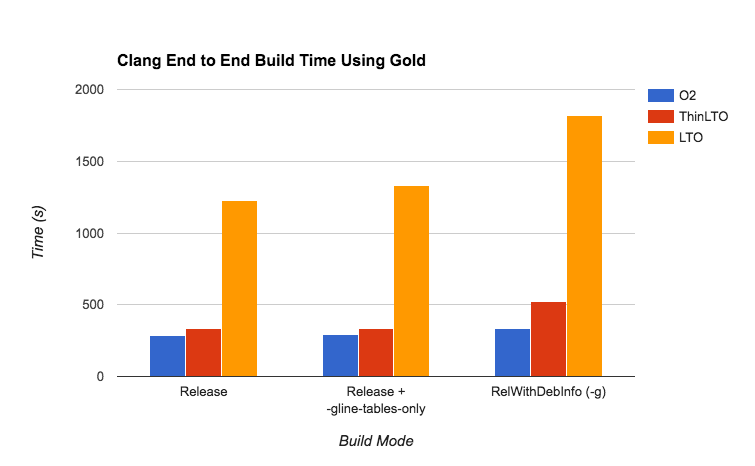
\includegraphics[width=0.8\textwidth]{build_time.png}
  \caption{Разлика у времену превођења програма
   између ThinLTO и регуларне оптимизације током линковања }
  \label{fig:grafikon}
\end{figure}

На слици 4.4 видимо да је време компајлирања програма са ThinLTO оптимизацијом
јако слично времену превођења без оптимизације током линковања.
Осетнија разлика између ова два начина компајлирања је приликом компајлирања
програма који има информације потребне за дебаговање, али у току су унапређења
у овом пољу, па се очекује смањење ове разлике у будућности.
Што се тиче регуларне оптимизације током линковања, компајлирање програма
је далеко спорије него код ThinLTO-а у сваком измереном случају.
 
\begin{figure}[!ht]
  \centering
  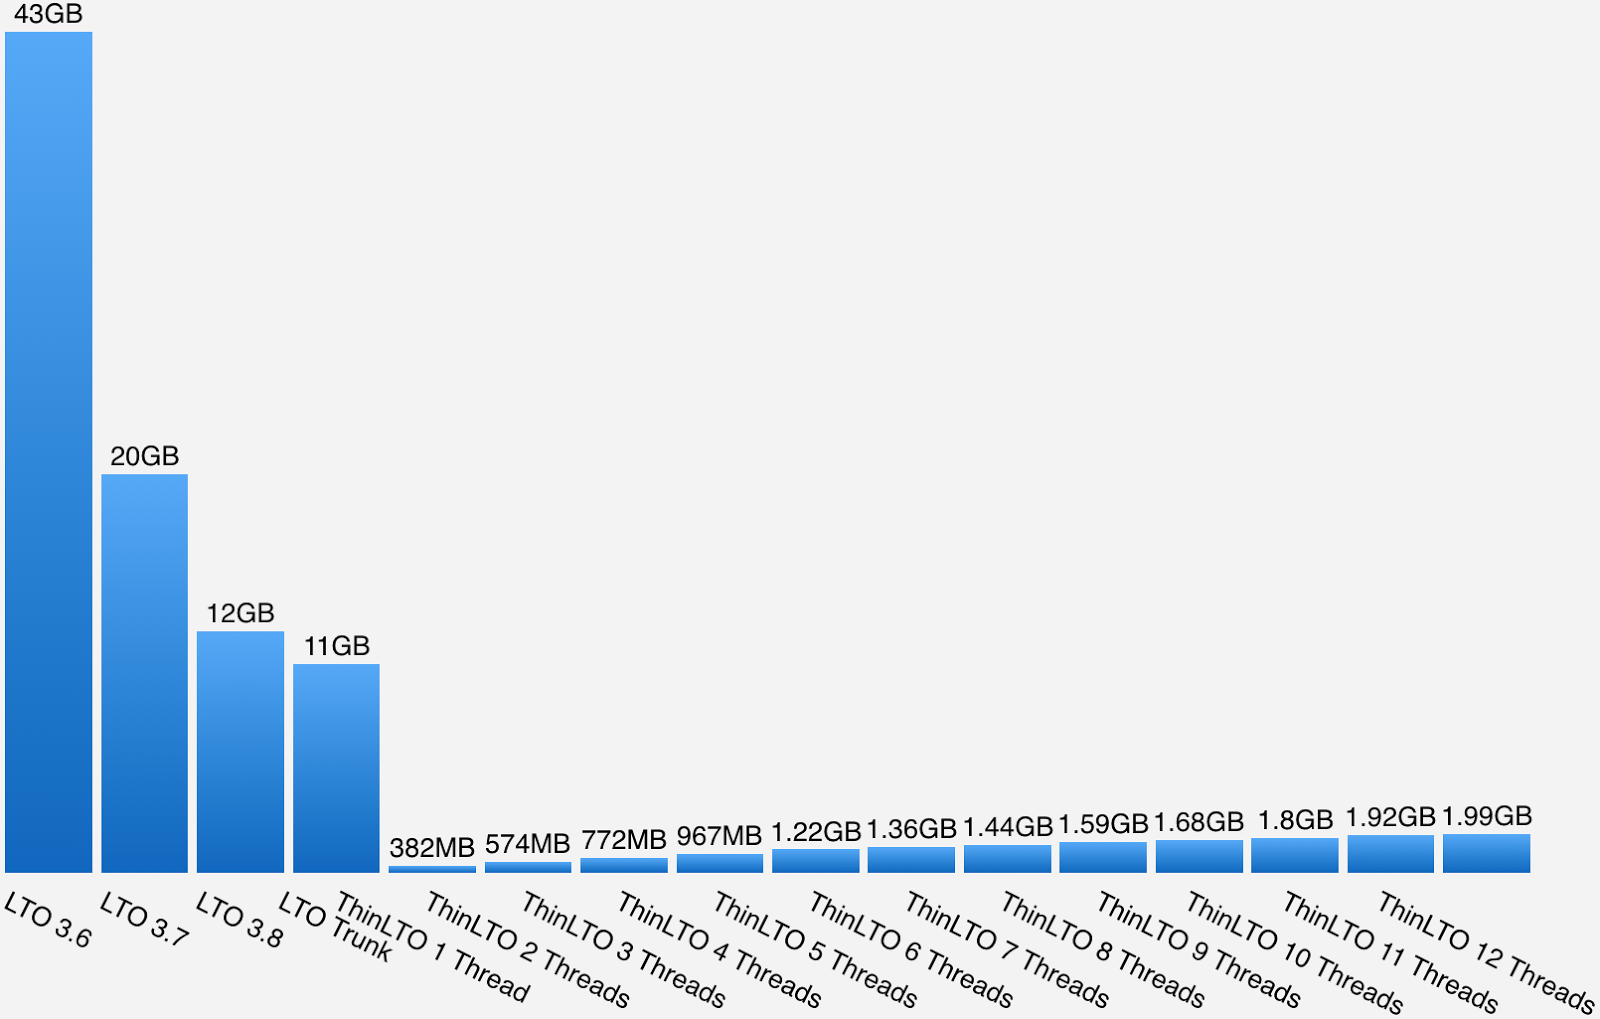
\includegraphics[width=0.8\textwidth]{memory.png}
  \caption{Разлика у меморијским захтевима
   између ThinLTO и регуларне оптимизације током линковања }
  \label{fig:grafikon}
\end{figure}

Јасно се види на слици 4.5 да је меморијска потрошња регуларне оптимизације
током линковања далеко већа од меморијске потрошње ThinLTO-а.
Такође, видимо да због огромне потрошње меморије за регуларну оптимизацију
током линковања морамо да имам далеко јачи хардвер него за  ThinLTO-а, да би уопште
превели програм.

\chapter{Алат за визуализацију промена}

Алат виртуализује промене унутар LLVM међурепрезентације програма 
преведеног са и без оптимизације целовитог програма.
Инспирација за овај алат био је compiler explorer[22].
Идеја иза compiler explorerа била је приказивање одговарајућих асемблерских
инструкција за сваку линију изворног к\^{o}да.
Ова функционалност је корисна јер програмер тако има увид у к\^{o}д који је 
компајлер изгенерисао за њега и евентуално може да пронађе неку грешку у 
изворном к\^{o}ду која је видљива након оптимизација.
Касније, у compiler explorer додата је подршка и за приказ LLVM међурепрезентације,
јер је она разумљивија од конкретног асемблерског језика и садржи више опција
за дебаговање.
Compiler explorer приказује промене у контексту једне јединице транслације,
 што значи да к\^{o}д мора да се успешно компајлира али не мора да се линкује. 
Са друге стране, алат за виртуализацију имплементиран за потребе овог рада,
приказује разлике у међурепрезентацијама у извршном фајлу, који је компајлиран
са и без оптимизације целовитог програма.
За разлику од compiler explorer-а за коришћење овог алата неопходно је да сви
улазни фајлови буду успешно линковани, али због тога он може да прикаже 
међурепрезентације извршних фајлова.
Алат повезује линије изворног к\^{o}да са одговарајућим линијама у LLVM 
међурепрезентацији, одговарајуће линије су приказане истом бојом.
Такође, постоји опција приказивања diff-a[24] између међурепрезентација са и без
активне оптимизације целовитог програма.
Тренутно, подржани су искључиво програми писани у програмском језику C++.
Изворни  к\^{o}д алата може се наћи на адреси[23].

Захтеви за покретање алата:
\begin{enumerate}
\item оперативни систем Linux
\item python3
\item python3-tk
\item clang
\item llvm
\item wllvm
\item kompare
\end{enumerate}

Пример покретања алата:

\begin{lstlisting}[frame=single]
python3 -i {putanja_do_foldera_sa_.cpp_fajlovima}
-o {nivo_optimizacije('0', '1', '2', '3', '4',
                     'z', 'g', 'z', 'fast)}

\end{lstlisting}

Алат је написан у програмском језику Python и садржи две главне функционалности.

Прва функционалност је приказ LLVM међурепрезентације са и без активне оптимизације
целовитог програма као и њихово мапирање са линијама у изворном к\^{o}ду.
Мапирање је имплементирано тако  једној линији у изворном к\^{o}ду придружује
одговарајуће линије у међурепрезентацијама.
Свако мапирање је обојено различитом бојом и обојене су само оне линије у изворном
к\^{o}ду које су се после свих оптимизација превеле у одговарајућу међурепрезентацију
 (линије које су избачене се не боје).
 
Друга функционалност је приказивање графичког diff-a унутар алата kompare[25].
Класичан diff не би имао много смисла, зато су игнорисана имена променљивих
и извршено је енкодирање "име фајла:линија изворног  к\^{o}да:LLVMIR".
Име фајла је обавезно да би направили разлику између истих линија  к\^{o}да у две различите јединице транслације.
Такође, занемарени су неки коментари и атрибути.
У diff-у на крају имамо приказне оригиналне линије унутар међурепрезентације, 
уколико су енкодиране линије различите у оптимизованој и неоптимизованој верзији.
Уколико су енкодиране линије исте, онда приказујемо енкодиране линије.

У наставку ћемо приказати излаз алата над следећим фајловима.

\begin{lstlisting}[frame=single]
\\ a.hpp
int calculate(int num);

\\a.cpp
#include "a.hpp"


int g_i = 1;

int calculate(int a){
    if (g_i){
        return a * a;
    }
    else{
       return a + a;
    }
    
}

\\ main.cpp
#include "a.hpp"
#include <iostream>

int main(){
    int n;
    std::cin >> n;
    
    int result = 0;

    for (int i = 0 ; i < n; i++){
        result += calculate(i);
    }

    return result;
}
Primer 5.1

\end{lstlisting}

Када покренемо алат добијамо следећу слику:

\begin{figure}[!ht]
  \centering
  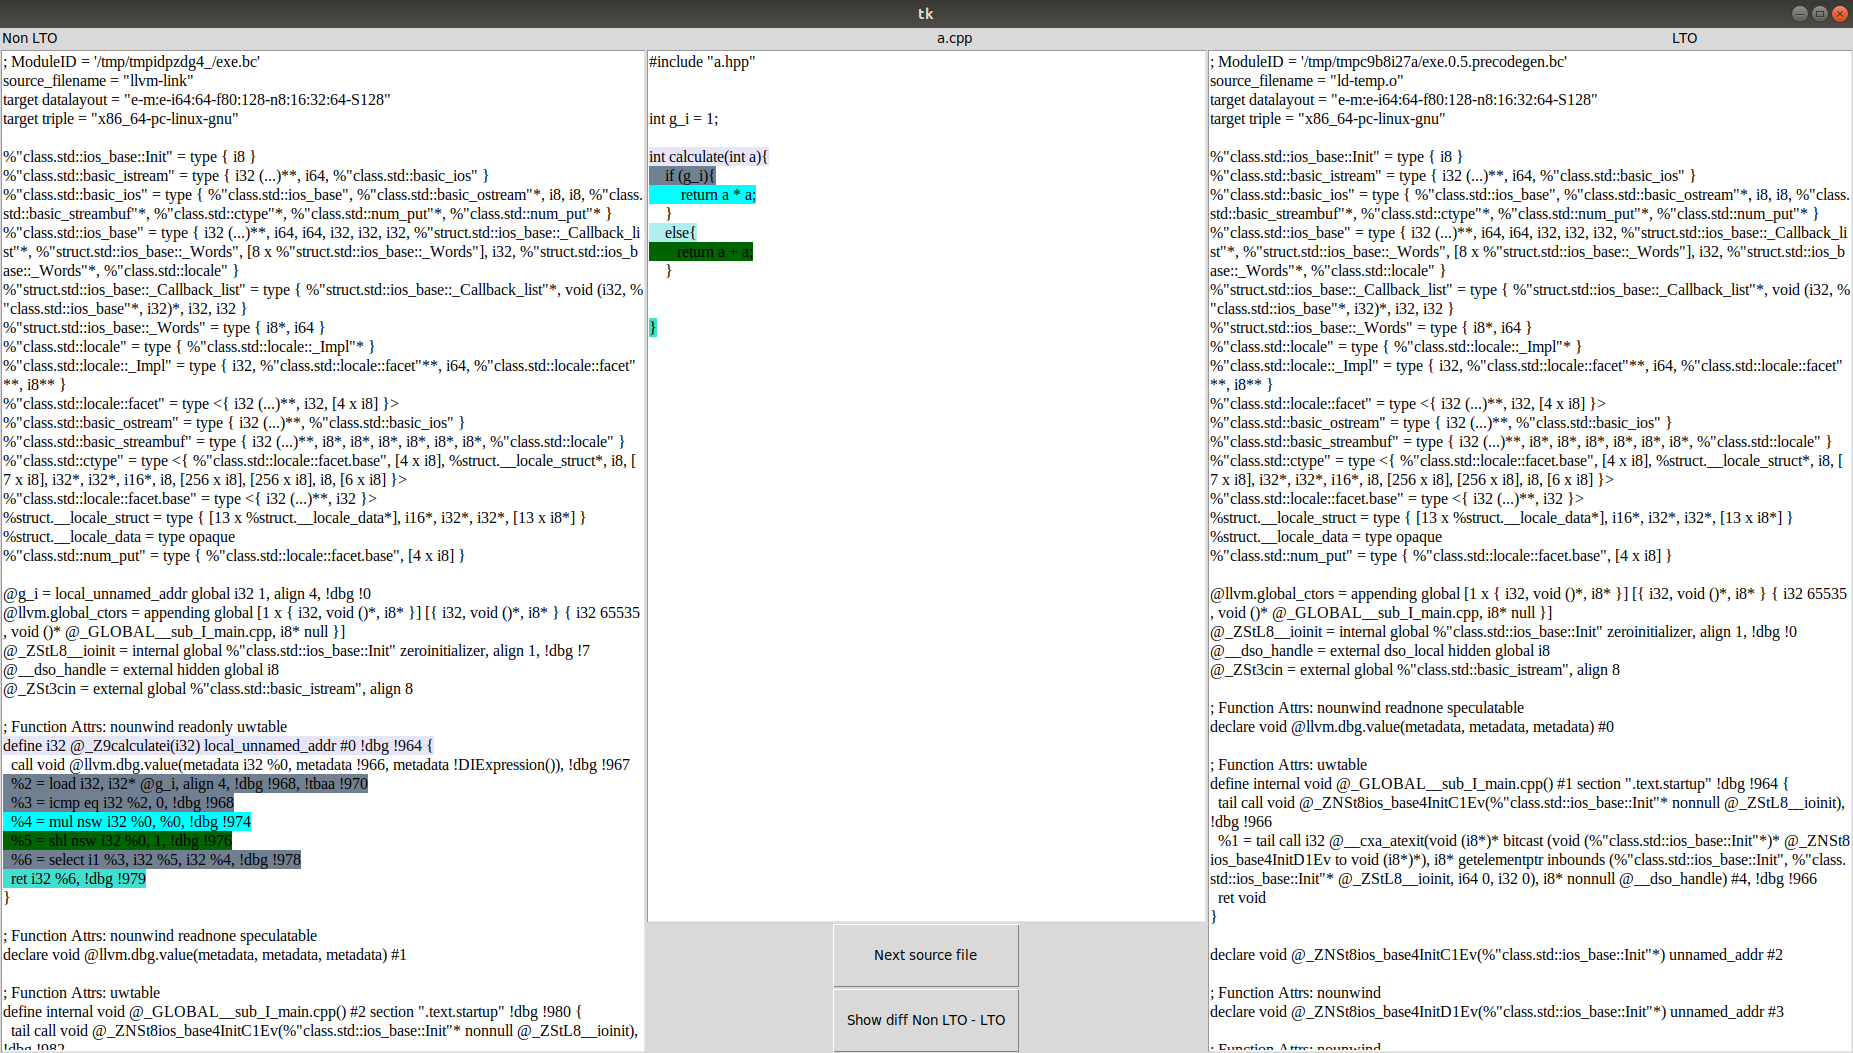
\includegraphics[width=0.8\textwidth]{a_cpp.png}
  \caption{Први изворни фајл }
  \label{fig:grafikon}
\end{figure}

У средњем прозору видимо да је тренутни изворни фајл, који повезујемо са одговарајућим
међурепрезензацијама, фајл a.cpp.
Са његове леве стране налази се прозор међурепрезентације где није извршена оптимизација
целовитог програма, и обојене истим бојама одговарајуће линије у изворном и
LLVM фајлу.
Са десне стране се налази прозор са оптимизованом међурепрезентацијом где видимо
да ништа није обојено, то је зато што је цео к\^{o}д  a.cpp фајла оптимизован
и не налази се у извршном фајлу.

Кликом на дугме Next source file, приказује се main.cpp фајл и одговарајуће 
мапирање линија.
\begin{figure}[!ht]
  \centering
  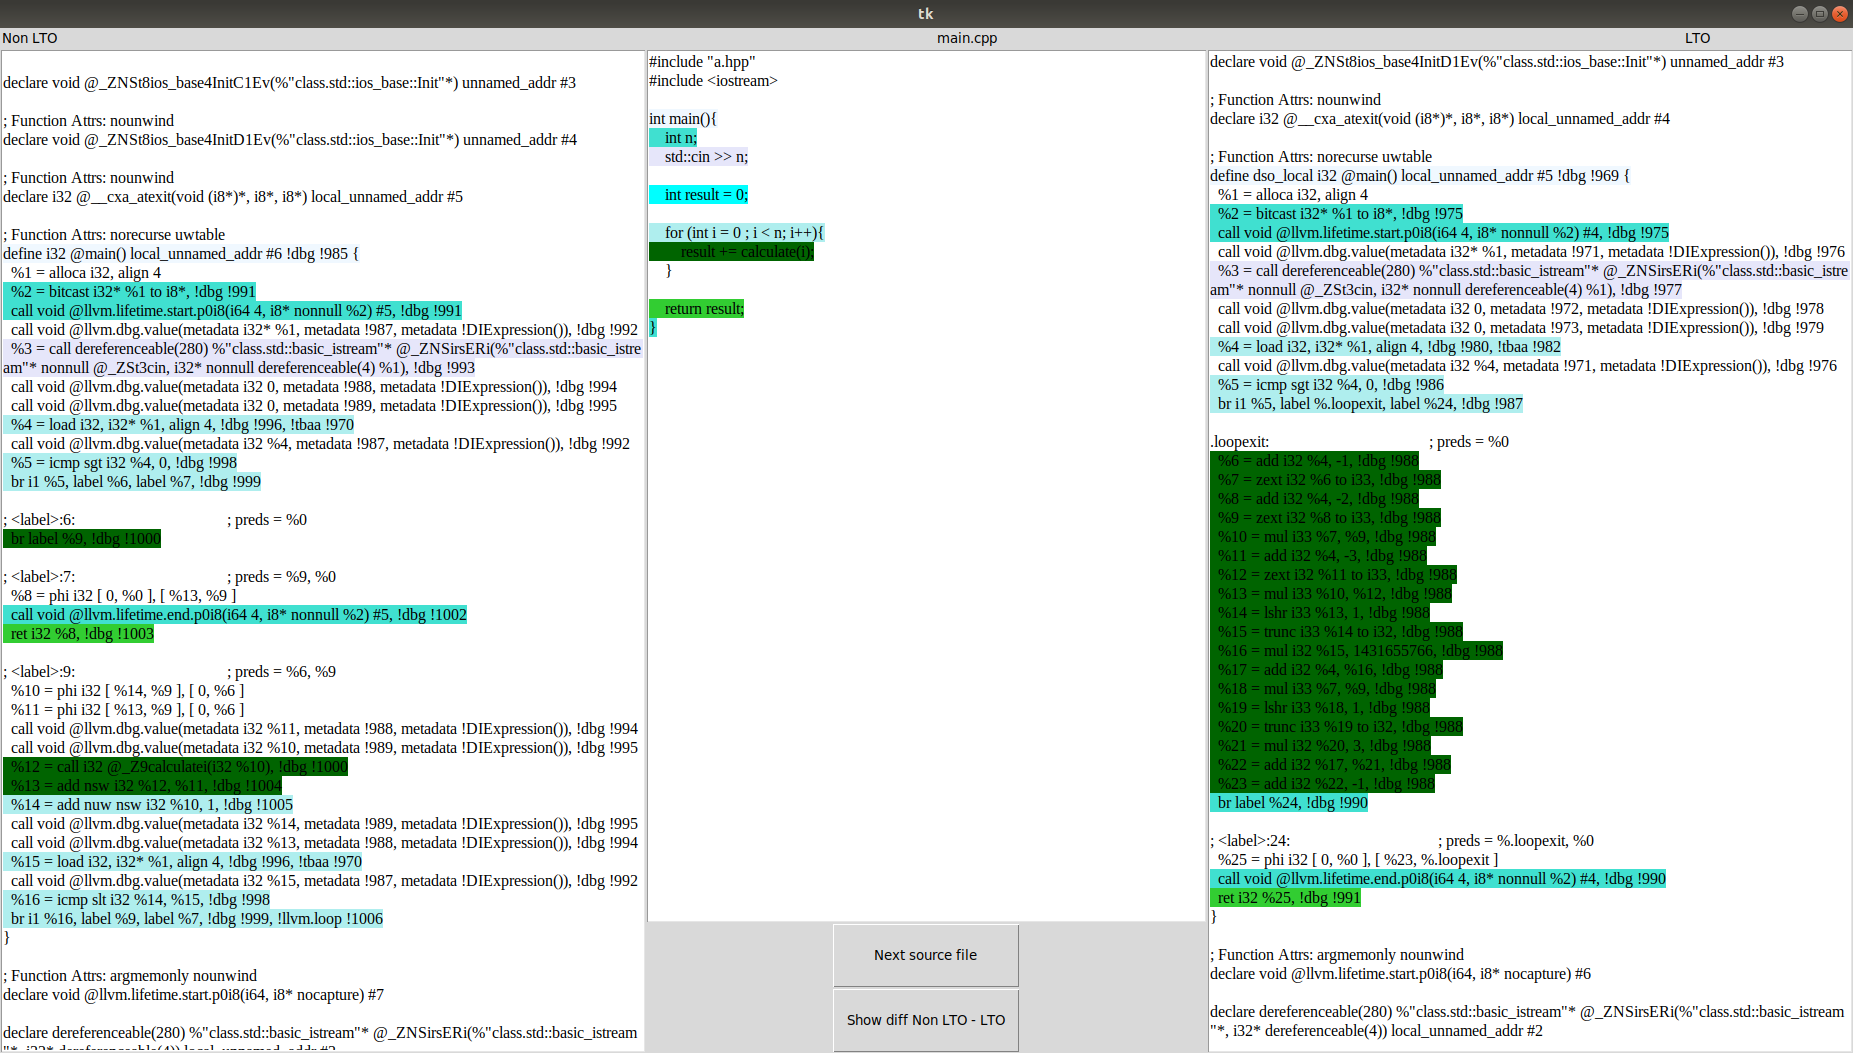
\includegraphics[width=0.8\textwidth]{main_cpp.png}
  \caption{Други изворни фајл }
  \label{fig:grafikon}
\end{figure}
Наравно, више се не приказују мапирања из претходног изворног фајла, већ само из
тренутног.

Кликом на дугме Show diff добијамо приказ разлика између неоптимизоване и оптимизоване
верзије, приказане у алату kompare.
\begin{figure}[!ht]
  \centering
  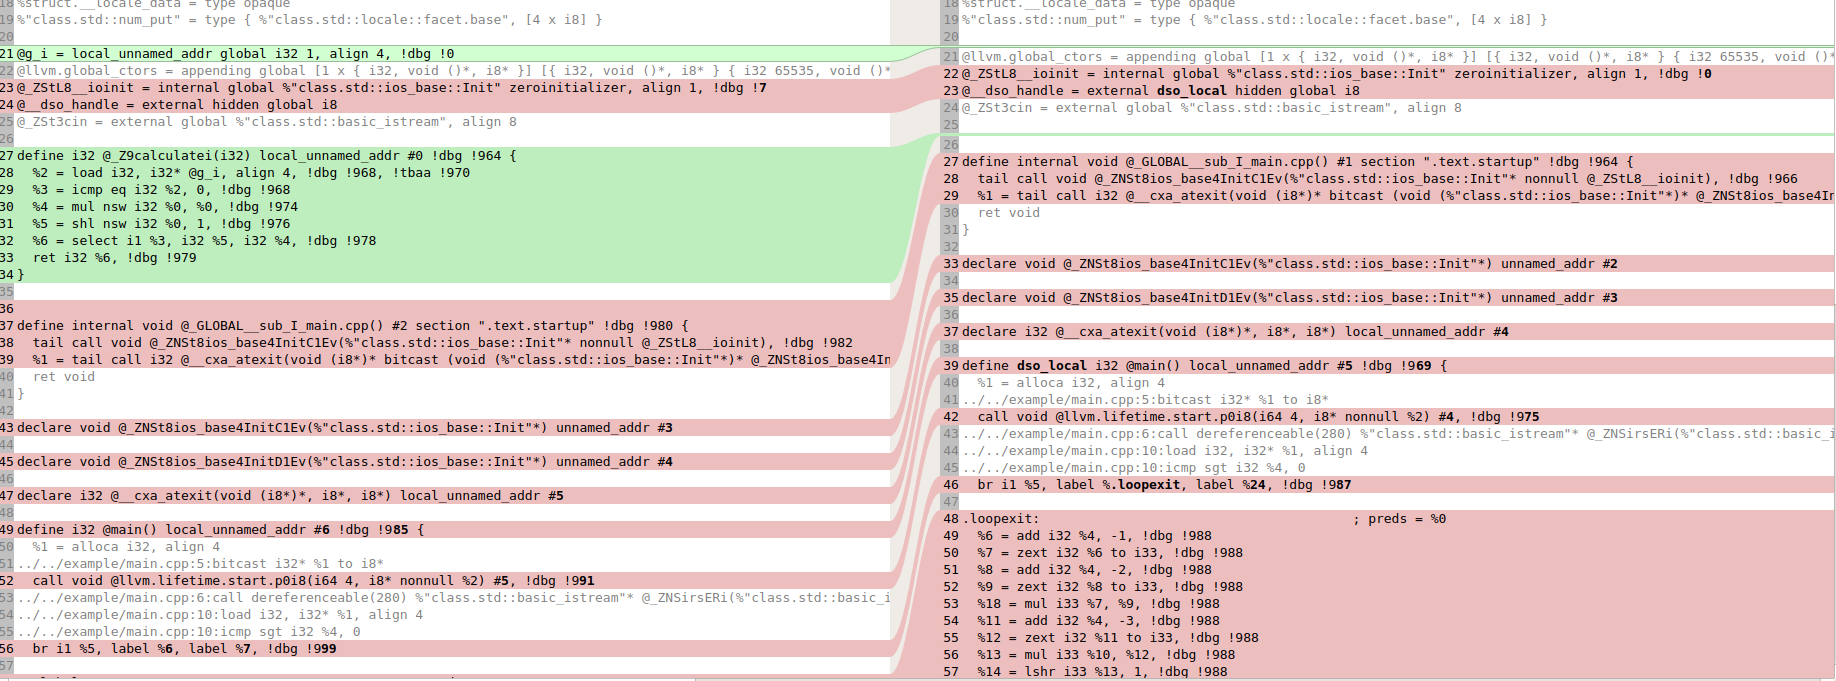
\includegraphics[width=0.8\textwidth]{diff_1.png}
  \caption{diff прва слика }
  \label{fig:grafikon}
\end{figure}
\begin{figure}[!ht]
  \centering
  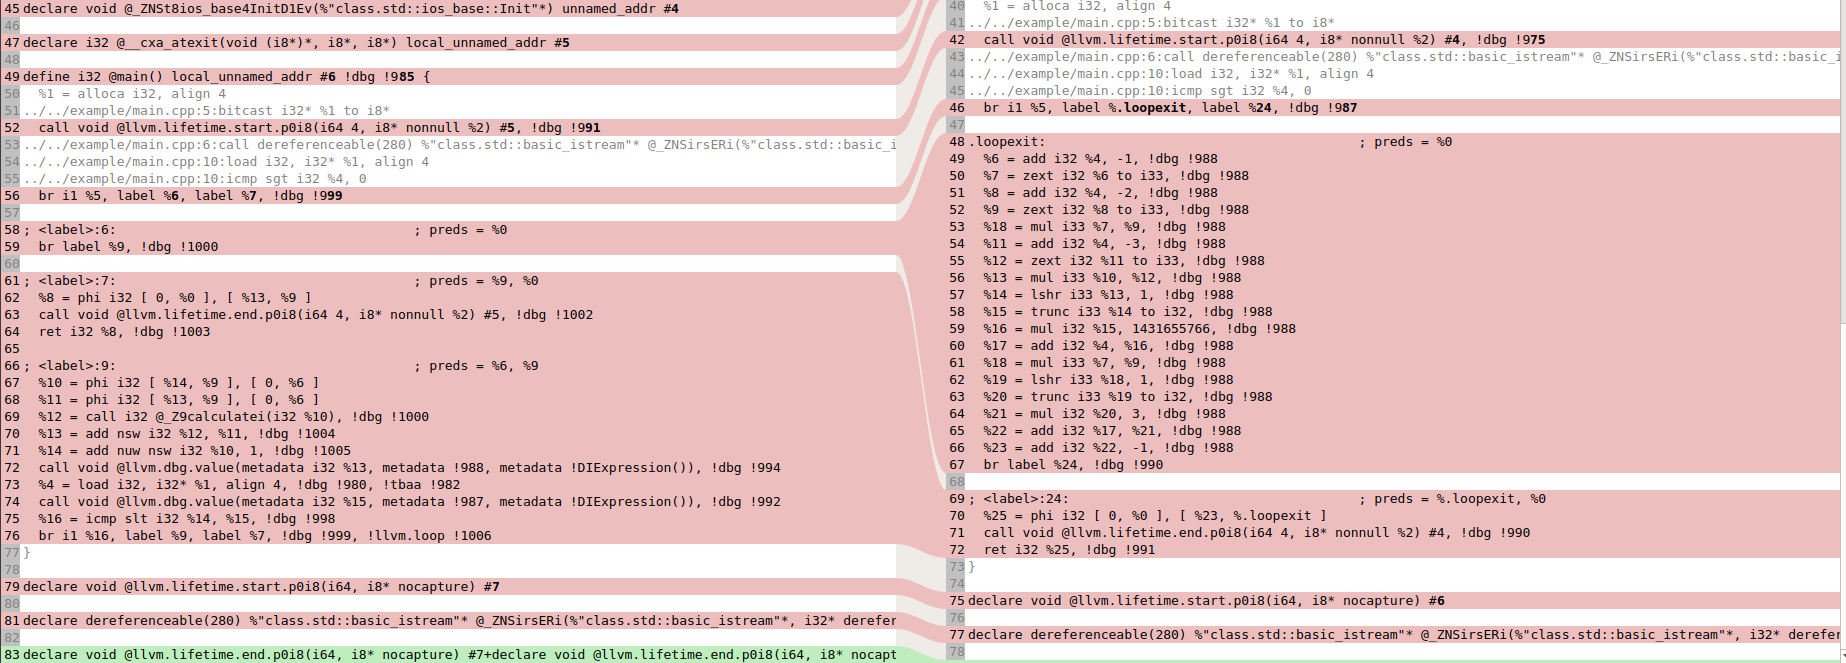
\includegraphics[width=0.8\textwidth]{diff_2.png}
  \caption{diff друга слика }
  \label{fig:grafikon}
\end{figure}
На слици 5.4 на 55. линији видимо пример енкодирања. 
Видимо да је та линија из фајла main.cpp и да је то десета линија у том фајлу.
И остале линије су енкодиране на сличан начин, само нису једнаке па користимо
њихове оригиналне верзије.

У примеру 5.1 видимо да је са активном оптимизацијом целовитог програма,
елиминисана глобална променљива g{\_}i  као и функција calculate.
Затим видимо и разлике у функцији main. 
Због тога што не види тело функције у верзији без активне оптимизације целовитог
програма, компајлер генерише к\^{o}д који позива функцију calculate.
У верзији са активном оптимизацијом целовитог програма, видимо не само да је функција
calculate инлајнована, већ је избрисан део функције који никада није доступан
јер је вредност глобалне променљиве увек 1, а то се може видети тек после процеса
линковања.
Taкође, видимо да је због инлајновања извршена и оптимизација петље, јер алат за
оптимизацију схвата шта рачунамо и извршава израчунавање без потребе за петљом.

% ------------------------------------------------------------------------------
\chapter{Закључак}
% ------------------------------------------------------------------------------
У раду је представљена LLVM компајлерска инфраструктура са посебним акцентом
на оптимизацију целовитог програма.
Видели смо да оптимизација целовитог програма доноси нека значајна побољшања
што се тиче времена извршавања и смањивања величине извршног фајла, али
са ценом у повећању времена потребном за превођење програма као и меморијско
заузеће током тог процеса.
Ови проблеми су донекле решени новим приступом у оптимизацији целовитог програма
ThinLTO, али уз нешто лошије перфомансе добијеног извршног фајла.
Додатно, у раду је имплементиран алат који визуализује промене између
међурепрезентација преведених са и без активне оптимизације целовитог програма,
што даје увид програмеру у генерисани компајлерски к\^{o}д.

У будућности LLVM заједница ће активно наставити на решавању проблема код 
оба приступа.
Такође, оптимизација целовитог програма се може користити за детекцију недефинисаног
понашања, када компајлер нема увид у цео к\^{o}д у јединици транслације и без
активне оптимизације целовитог програма компајлер не може програмеру да укаже
на грешку, чак и када су сва обавештења укључена (-Wall).
У gcc компајлеру је ова подршка имплементирана, што можемо видети у раду
Undefined behavior in theory and practice[26], тако да се у будућности ова
функционалност очекује и у clang компајлеру.



% ==============================================================================
% Završni deo teze i prilozi
\backmatter
% ==============================================================================
\chapter{Литература}
[1] LLVM Compiler Infrastructure -- https://llvm.org/docs/index.html \\

[2] LLVM Language Reference Manual -- https://llvm.org/docs/LangRef.html \\

[3] SSA Form -- https://en.wikipedia.org/wiki/Static{\_}single{\_}assignment{\_}form \\
 
[4] RISC -- https://en.wikipedia.org/wiki/Reduced{\_}instruction{\_}set{\_}computer \\

[5] Abstract Syntax tree -- https://en.wikipedia.org/wiki/Abstract{\_}syntax{\_}tree \\

[6] Optimizer -- https://llvm.org/docs/CommandGuide/opt.html \\

[7] LLVM Code Generator -- https://llvm.org/docs/CodeGenerator.html \\

[8] Just In Time Compilation  -- https://en.wikipedia.org/wiki/Just-in-time{\_}compilation \\

[9] Unity build -- https://en.wikipedia.org/wiki/Unity{\_}build \\ 

[10] Link Time Optimization -- https://llvm.org/docs/LinkTimeOptimization.html \\

[11] libLTO -- https://llvm.org/docs/LinkTimeOptimization.html{\#}liblto \\

[12] Gold linker -- https://llvm.org/docs/GoldPlugin.html \\

[13] llvm-link -- https://llvm.org/docs/CommandGuide/llvm-link.html \\

[14] Function inlining -- https://www.cs.cornell.edu/courses/cs6120/2019fa/blog/llvm-function-inlining/ \\

[15] Indirect branch instructions -- https://en.wikipedia.org/wiki/Indirect{\_}branch \\

[16] Dead code elimination -- https://en.wikipedia.org/wiki/Dead{\_}code{\_}elimination \\

[17] Devirtualization -- https://blog.llvm.org/2017/03/devirtualization-in-llvm-and-clang.html \\

[18] Internal linkage -- https://www.learncpp.com/cpp-tutorial/internal-linkage/ \\

[19] Unnamed namespace -- https://www.ibm.com/docs/en/i/7.3?topic=only-unnamed-namespaces-c \\

[20] ThinLTO -- https://clang.llvm.org/docs/ThinLTO.html \\

[21] http://blog.llvm.org/2016/06/thinlto-scalable-and-incremental-lto.html \\

[22] https://godbolt.org/ \\

[23] https://github.com/filipl41/master \\

[24] Diff -- https://en.wikipedia.org/wiki/Diff \\

[25] Kompare -- https://apps.kde.org/kompare/ \\

[26] Undefined behavior in theory and practice -- https://queue.acm.org/detail.cfm?id=3468263

\end{document}